\documentclass[a4paper, 11pt]{book}
\usepackage[utf8]{inputenc}
\usepackage{mathtools, amssymb, graphicx, amsmath, epstopdf, amsthm, mdframed}
\usepackage{xcolor}

\title{Notes on Information Theory}
\author{Cristian Di Pietrantonio, Michele Laurenti}

%PLEASE: see the macros defined and use them!

\newtheorem{prop}{Proposition}
\newtheorem{definition}{Definition}
\newtheorem{thm}{Theorem}
\newtheorem{obs}{Observation}
\newtheorem{lem}{Lemma}
\newtheorem{cor}{Corollary}

% math symbols

\newcommand{\M}{\mathcal{M}}
\newcommand{\X}{\mathcal{X}}
\newcommand{\Y}{\mathcal{Y}}

\newcommand{\Tau}{\mathrm{T}} % Capital Tau

\newcommand{\ie}{\textit{i.e.}, }

\newcommand{\xset}{\X}
\newcommand{\msgset}{\M} % the set of all messages
\newcommand{\yset}{\Y}
\newcommand{\cwset}{\mathcal{C}_n} % codewords set

\newcommand{\chrom}[1]{X(#1)}

\newcommand{\str}[1]{\underline{#1}} % string/vector
\newcommand{\zero}{\str{0}} % zero vector

\newcommand{\Reals}{\mathbb{R}}
\newcommand{\Naturals}{\mathbb{N}}

\newcommand{\abs}[1]{\left|{#1}\right|}
\newcommand{\floor}[1]{\left\lfloor{#1}\right\rfloor}
\newcommand{\ceil}[1]{\left\lceil{#1}\right\rceil}

\newcommand{\im}{\text{Im}} % image of linear application

\newcommand{\sfrac}{\frac}
\newcommand{\ifrac}[2]{\frac{#1}{#2}} % Inline fraction

\newcommand{\hball}[2]{B_H\left(#1, #2\right)} % the Hamming ball
\newcommand{\hdist}[1]{d_H \left({#1}\right)} % Hamming distance
\newcommand{\hweight}[1]{w_H\left(#1\right)} % Hamming weight

\renewcommand{\pref}{\leftarrowtail} % is prefix relation
\newcommand{\prol}[1]{Y_L(#1)} % all the strings that have x as prefix

\newcommand{\supp}{\text{Supp}_w} % support


\begin{document}
	\frontmatter
	\maketitle
	%\chapter{Preface}

These are notes taken during the Information Theory course held by Professor J\'anos K\"{o}rner at La Sapienza, University of Rome (Class of 2016).
	
	\mainmatter
	\chapter{Introduction}
Information Theory is born from one man, Cloude Shannon (1926 - 2001). It has to do with probability, algebra, coding theory, ergodic theory and appears in daily life. 

\begin{itemize}
	\item Tom Cover, Joy Thomas, Information Theory, Wiley;
	\item IT: cooling theorems for discrete memoryless systems, Korner;
	\item IT, Robert Ash.
\end{itemize}

%In communication you want to be understood, but you also want to avoid redundancy and words tend to be lengthy; there is a conflict of interest. Why some words are short and others are long? Short words encode common abstract pictures whereas long words must carry the whole information not available in common knowledge. Suggested readings: 

%\section{Base concepts and considerations}
%Define $\msgset$ as the finite set of all messages over an alphabet $\Sigma$. A message $m$ is an element of $\msgset$. Hartley, who introduced this concept before Shannon, stated that the maximum amount of information is equal to $\log_2 |\msgset|$, since one can identify elements of $\msgset$ with binary strings of length $\log_2 |\msgset|$. Formally $$\msgset \sim \{0, 1\}^{\left\lceil\log_2 |\msgset|\right\rceil} $$ and $$ m \sim \Delta \in \{0, 1\}^{\left\lceil\log_2 |\msgset|\right\rceil}.$$

%One can think of $\Delta$ as a sequence of $\log_2 |\msgset|$ binary questions that identify an element in $\msgset$. A single unit of information is a $0$ or $1$ (Binary Information Theory). In the \emph{20 question game}, where you need to minimize the number of questions to guess what a person thinks, is given a probability distribution $P$ over $\msgset$ (denoted from now on as $P|M$) s.t. $P(m) \geq 0,\ \forall m \in \msgset$ and $\sum_{m \in \msgset} P(m) = 1$. The questions can be designed to make the game as short as possible if $P$ is known.

%Must be noted that $|\underline{x}| = i \Leftrightarrow \underline{x} \in \{0, 1\}^{i}$. The number of questions asked on average must be minimized. Let $f: \msgset \rightarrow \{0, 1\}^*$, in other words a mapping from the message set to the sequences of answers to find the message then we want to minimize 
%\begin{equation} \label{eq:problen}
%\sum_{m \in \msgset} P(m) |f(m)|.
%\end{equation} 
%This equation is tied only to the probability distribution, not to the set or the questions. If $P$ is uniform then the Expression \ref{eq:problen} is equal to $\left\lceil\log_2 |\msgset|\right\rceil$. The function $f$ is called \emph{code}. The code is not always invertible.

%Communication happens at a distance, otherwise it would be trivial. There is some device that makes communication possible; the channel is not perfect. The noise is random, modeled through a probability distribution. The information source is not predictable either and will have its own probability distribution too. Encoding and decoding must be optimized to make communications short to reduce loss of information, and to reliably transmit, i.e. the receiver is reasonably sure that it gets what was sent. The two aspects are in contrast, you need and optimal trade-off. Usually partners in communication are separated in space and communication takes place in time. Sometimes in computer science the opposite thing happens: communication is storing information in space to retrieve it later in time. Sometimes you want to shorten the communication time, sometimes the space communication takes.
	%October 2016, the 4th
\chapter{The Hamming Ball}

This Chapter introduces an important concept: the Hamming Ball.

\section{Hamming space}

A \emph{space} is a set that has structure.
The set $\{0,1\}^{n}$ of binary strings of length $n$ can be made into a metric space.
To make it a metric space we have define a metric (or distance) on it.

A metric over set $\X$ is a function $d: \X \times \X \rightarrow \Reals$ that has the following properties:
\begin{enumerate}
	\item it's greater than zero, \ie $d(x, y) \geq 0$ $\forall (x, y) \in \X \times \X$, with equality when its arguments are the same, \ie $d(x, y) = 0 \iff x = y$;
	\item it's symmetric, \ie $d(x, y) = d(y, x)$ $\forall (x, y) \in \X \times \X$;
	\item it satisfies the triangular inequality, \ie $d(x, y) \leq d(x, z) + d(z, y)$.
\end{enumerate}

For $\{0,1\}^{n}$ we define the \emph{Hamming metric}.
Consider two strings, $\str{x}, \str{y}  \in \{0, 1\}^n$.
Then their Hamming distance is defined as
\begin{equation}
	\hdist{\str{x}, \str{y}} = \abs{\{i : x_i \not= y_i\}}.
\end{equation}

The first two properties are trivial to see.
For the third property, consider three strings $\str{x}$, $\str{y}$, $\str{z} \in \{0,1\}^n$.
Let $D = \{i : x_i \not= y_i\}$ be the set of coordinates where they differ.
If $i \in D$, we have $x_{i} \neq y_{i}$.
What can happen to $z_{i}$?
Either $z_{i} \neq x_{i}$ or $z_{i} \neq y_{i}$.
If $i \not\in D$, $z_{i}$ is either equal to both $x_{i}$ and $y_{i}$, or it differs from both of them.
Thus, $\hdist{x_{i},y_{i}} \le \hdist{x_{i},z_{i}} + \hdist{z_{i},y_{i}}$ for all $i$.

Now, since the Hamming metric is additive, we have
\begin{align*}
	\hdist{\str{x},\str{y}} & =
	\sum_{i = 1}^n \hdist{x_i,y_i} \\
	& \le
	\sum_{i = 1}^n \hdist{x_i,z_i} +
	\sum_{i = 1}^n \hdist{z_i,y_i}
	=
	\hdist{\str{x},\str{z}} +
	\hdist{\str{z},\str{y}}
\end{align*}
which gives us the triangular inequality.

In general,  a distance is extended to a product space by summing the distances of the single components, as happens for the Hamming metric.

Consider a storage device that has $n$ cells, each containing either $0$ or $1$.
Suppose memory decays with time in some unknown way.
After some time the string memorised in the device will be different.
The Hamming distance tells us how much different.

If a string $\str{x}$ has been changed no more than $r$ times to become $\str{y}$, then $d_H(\str{x}, \str{y}) \leq r$.
We say that $\str{y}$ is in a \emph{Hamming Ball} of radius $r$ around $\str{x}$.

\begin{definition}[Hamming Ball]
	The Hamming Ball of radius $r$ and centre $\str{x}$ is the set
	\begin{equation}
		\hball{\str{x}}{r} = \{\str{y} : \hdist{\str{x},\str{y}} \leq r\}.
	\end{equation}
\end{definition}

\begin{obs}
	$r$ needs not to be an integer, but for $r \in \Reals$ it holds that
	\begin{equation*}
		\hball{\str{x}}{r} = \hball{\str{x}}{\floor{r}}.
	\end{equation*}
\end{obs}

Note that $\{0,1\}^{n}$ is a Hamming Ball of radius $n$, for any centre.

If you have a ball that is not the whole space, then the centre of this ball is unique.

What we can say about the size of a generic Hamming Ball $\hball{\str{x}}{r}$, with $r > 0$?
For the sake of simplicity, consider $\hball{\zero}{r}$, where $\zero$ is the string of all zeros.
Then the size of this Hamming Ball is
\begin{equation}\label{eq:volume}
	\abs{\hball{\zero}{r}} = \sum_{i = 0}^{\floor{r}} \binom{n}{i}
\end{equation}
\ie the number of ways in which we can flip to 1 up to $r$ bits.

\begin{definition}[Hamming weight]
	The Hamming weight of a string is its distance from $\zero$, \ie
	\begin{equation}
	\hweight{\str{x}} = \hdist{\zero,\str{x}}.
	\end{equation}
\end{definition}

If one subtracts $\hball{\str{x}}{r}$ to $\{0, 1\}^n$, then the result is also an Hamming ball.

To see this, consider a string $\str{y}$ that is not in $\hball{\zero}{r}$.
Then it must be that $\hweight{\str{y}} > r$.
What is its distance from the string of all ones, \ie $\hdist{\str{y},\str{1}}$?
One can see that $\hdist{\str{y},\str{1}} = n - \hweight{\str{y}}$, since $\hdist{\zero,\str{x}} + \hdist{\str{1},\str{x}} \ge \hdist{\str{0},\str{1}} = n$.
More in general we can bound the distance as $\hdist{\str{y},\str{1}} < n - r$, or $\hdist{\str{y},\str{1}} \le n - (r+1)$, which means that $\str{y}$ is in a Hamming Ball of radius $n - (r+1)$ with centre $\str{1}$.

From it we derive the following result:
\begin{equation}
	\overline{\hball{\str{0}}{n}} = \{0,1\}^{n} \setminus \hball{\str{0}}{n} = \hball{\str{1}}{n - (r+1)}.
\end{equation}
In other words the Hamming space can be partitioned into two Hamming balls.

If $n$ is odd, the Hamming space can be partitioned in the following way: $$\{0, 1\}^n = \hball{0}{\floor{\frac{n}{2}}} \cup \hball{1}{\floor{\frac{n}{2}}}$$
The Hamming space cannot be partitioned into three balls.
In how many balls can $\{0, 1\}^n$ be partitioned?
It cannot partitioned be partitioned into $s$ balls with $3 \leq s \leq n + 1$ (this result has not been demonstrated).

\section{The volume of a Hamming ball}
We have seen that the volume of a generic Hamming ball is described by Equation \ref{eq:volume}. We can use the Pascal triangle to get a feeling about the order of magnitude of the Hamming ball. Consider the $n$th row in the triangle; since it is symmetric, if we split the row in half the sum of the terms of the first part is equal to the sum of the terms of the second part of the row. The volume of the greatest ball is $|\hball{0}{n}| = 2^n$. Instead, the volume of the ball with radius $n/2$ (in the triangle's point of split) is $\ifrac{2^n}{2} = 2^n2^{-1} = 2^{n-1}$. It follows, if $r \geq \ifrac{n}{2}$, that $2^{n-1} \leq |\hball{0}{r}| \leq 2^n$. Can we bound the volume for $r < \ifrac{n}{2}$?

\subsection{Entropy}
First we introduce the notion of \emph{entropy}. Entropy is a function $h: [0, 1] \rightarrow [0, 1]$ defined as follows:
\begin{equation}
	h(t) = t\log_2(\dfrac{1}{t}) + (1 - t)\log_2\left(\dfrac{1}{1-t}\right)
\end{equation}

The plot of $h$ looks like this:
\begin{figure}[h]
	\centering
	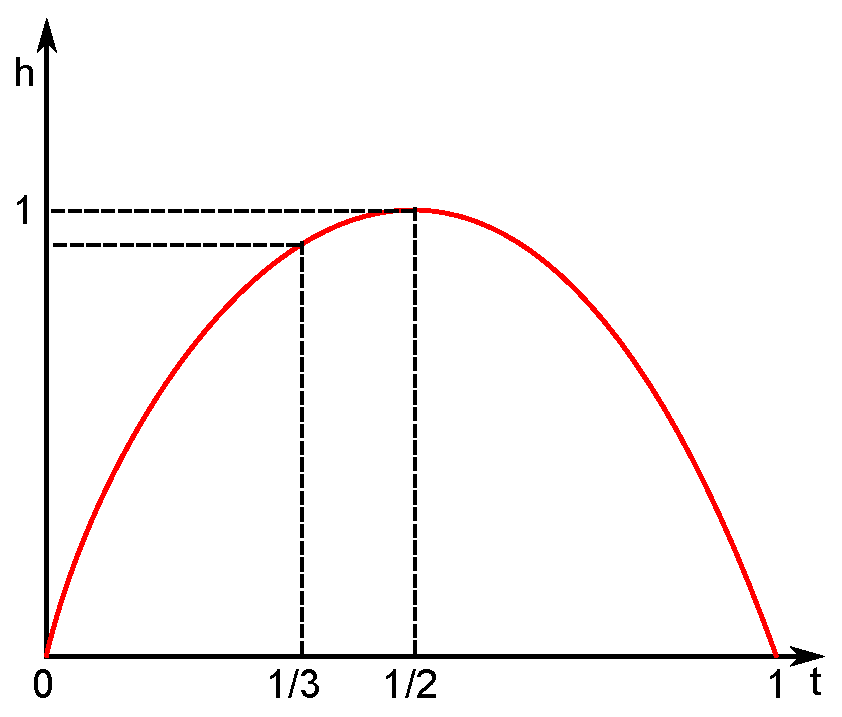
\includegraphics[width=0.6\linewidth]{pictures/ch01-i00.eps}
	\caption{The entropy function.}
\end{figure}

This function is not defined for the values $0$ and $1$. However, we have limits defined on these points and they are both $0$. So we artificially set $h(0) = 0$ and $h(1) = 0$. It is better to think about it as probability distribution $(t, 1 - t)$ and entropy is a number attached to it. Entropy measures symmetry and with $t = \ifrac{1}{2}$ we have maximum chaos (the future outcomes are equally likely).

\subsection{Lower and upper bounds}

\begin{thm}
	The upper bound on the volume of a Hamming ball, if $ r \leq \ifrac{n}{2}$, is
	$$|\hball{0}{r}| \leq 2^{nh\left(\sfrac{r}{n}\right)}$$
\end{thm}

In order to prove this theorem an analogy is introduced. Suppose there is a box with a number of chickens in it. We want to count those animals without withdrawing all of them out of the box. What can be done is to take the lightest one and measure its weight $w$; then also the weight $W$ of the box is measured. The number of the total chickens in the box can't be greater than $\ifrac{w}{W}$.\\

\noindent\textbf{Proof.} In this proof we will use a similar technique. Consider $\{0, 1\}^n$. We ``sparkle'' a substance on the strings in the set; this substance looks like probability, but it doesn't matter. Define the weight of $1$ and $0$ as 
$$P(1) = \dfrac{r}{n},\ P(0) = 1 - P(1).$$

Notice that is not an uniform distribution. Define the weight of a string as
$$P^n(\str{x}) = \prod_{i = 1}^n P(x_i).$$

If $A \subseteq \{0, 1\}^n$ then the weight of the set $A$ is $$P^n(A) = \sum_{\str{x} \in A} P^n(\str{x}).$$

$P^n(\{0, 1\}^n)$ is the total weight of the substance sparkled on the strings and it is the probability distribution of binomial. For this reason one can claim that
$$1 = P^n(\{0, 1\}^n) \geq P^n(\hball{0}{r}) = \sum_{\str{x} \in \hball{0}{r}} P^n(\str{x})$$

at this point we ``take out the lightest chicken'' and write
$$\sum_{\str{x} \in \hball{0}{r}} P^n(\str{x}) \geq |\hball{0}{r}| \cdot \min_{\str{x} \in \hball{0}{r}}P^n(\str{x})$$

Which are the lightest chickens? Because we assume $r \leq \ifrac{n}{2}$ then
$$r \leq \dfrac{n}{2} \Rightarrow P(1) = \dfrac{r}{n} \leq \dfrac{1}{2} \Rightarrow P(1) \leq P(0).$$
It follows that the the lightest strings are the ones on the border of the ball, with $r$ $1$'s. We now compute their weight.

\[\min_{\str{x} \in \hball{0}{r}}P^n(\str{x}) = [P(1)]^r\cdot[P(0)]^{n-r} = \] 
\[ = \left(\dfrac{r}{n}\right)^r \left(1 - \dfrac{r}{n}\right)^{n-r} = \]  \[ = \left(\dfrac{r}{n}\right)^{n\sfrac{r}{n}} \left(1 - \dfrac{r}{n}\right)^{n\left(1 - \sfrac{r}{n}\right)} =\]
\[ = [\left(\dfrac{r}{n}\right)^{\sfrac{r}{n}} \left(1 - \dfrac{r}{n}\right)^{\left(1 - \sfrac{r}{n}\right)}]^n =\] 
\[ =2^{n\log_2[\left(\sfrac{r}{n}\right)^{\sfrac{r}{n}}  \left(1 - \sfrac{r}{n}\right)^{\left(1 - \sfrac{r}{n}\right)}]} = \]
\[ =2^{n[\sfrac{r}{n}\log_2\sfrac{r}{n} + \left(1 - \sfrac{r}{n}\right)\log_2\left(1 - \sfrac{r}{n}\right)]} = 2^{-nh\left(\sfrac{r}{n}\right)}\]

So we have 

\[1 \geq |\hball{0}{r}| \dfrac{1}{2^{nh(\sfrac{r}{n})}} \Rightarrow |\hball{0}{r}| \leq 2^{nh\left(\sfrac{r}{n}\right)}\] 
\hfill$\Box$


\begin{thm}
	The lower bound on the volume of a Hamming ball, if $ r \leq \ifrac{n}{2}$, is
	$$|\hball{0}{r}| \geq \dfrac{1}{n+1}2^{nh(\sfrac{r}{n})}$$
\end{thm}

\noindent\textbf{Proof.} $$P(1) = \dfrac{r}{n},\ P(0) = 1 - P(1),\ P^n(\{0, 1\}^n) = 1.$$
Consider the set of all strings of length $n$ and partition it in the following way.
$$\Tau_q^n = \{\str{x}\ |\ \hweight{x} = q\},$$
obtaining $n +1$ classes. 
We know that $|\Tau_q^n| = \binom{n}{q}$; we are not interested in how many strings are in that set, but what is the total weight; we want to prove $$ |T_r| \geq \dfrac{1}{n+1}2^{nh\left(\sfrac{r}{n}\right)}.$$ There is not symmetry in the weight of the partitions so there is a weight $r$ so that
$$ \dfrac{P^n(\Tau_q)}{P^n(\Tau_r)} \leq 1,\ \forall q$$
In the formula above there are binomials we want to bound.

\begin{obs}
	$$\dfrac{k!}{l!} \leq k^{k-l}.$$
\end{obs}

\noindent\textbf{Proof}. We are going to prove this observation in two steps.
\begin{itemize}
	\item $k \geq l$. 
	$$\dfrac{k!}{l!} = \dfrac{k(k-1) \cdots l(l -1) \cdots 1}{l(l -1) \cdots 1} \leq k^{k-l}.$$
	
	\item $k < l$.
	$$\dfrac{k!}{l!} = \dfrac{k(k-1) \cdots 1}{l(l -1) \cdots k(k-1) \cdots 1} \leq \left(\dfrac{1}{k+1}\right)^{l-k} < \left(\dfrac{1}{k}\right)^{l-k} = k^{k-l}.$$
\end{itemize}
\hfill$\Box$

% Lesson5
Define $p = \ifrac{r}{n}$  so that we have a distribution $P(p, 1-p)$ that picks a set and concentrate the weight (probability) on it. We observe that the probability of each string in a class depends only on the number of $1$'s in it. So we can write

\[\dfrac{P^n(\Tau_q)}{P^n(\Tau_r)} = \dfrac{p^q(1-p)^{n-q}|\Tau_q|}{p^r(1-p)^{n-r}|\Tau_q|} = p^{q-r}(1-p)^{r-q} \dfrac{\frac{n!}{q!(n-q)!}}{\frac{n!}{r!(n-r)!}} = \]
\[ = p^{q-r}(1-p)^{r-q}\dfrac{r!}{q!}\dfrac{(n-r)!}{(n-q)!} \leq p^{q-r}(1-p)^{r-q}r^{r-q}(n-r)^{q-r} = \]

considering that $r = np$ it follows that

\[p^{q-r}(1-p)^{r-q} (np)^{r-q}[n(1-p)]^{q-r}= \] \[ = p^{q-r}(1-p)^{r-q}n^{r-q+q-r}p^{r-q}(1-p)^{q-r} = \]

\[ = p^{q-r + r-q}(1-p)^{r-q+q-r} = 1.\]

So we can write

\[1 = P^n(\{0,1\}^n) = P^n\left(\bigcup_{q=0}^nT_q\right) = \sum_{q=0}^nP^n(T_q)\leq(n+1) \max_qP^n(T_q) = \]

\[=(n+1)P^n(T_r) = (n + 1)|T_r|2^{-nh\sfrac{r}{n}}\]

From the previous result we know $|T_r| \geq \dfrac{1}{n+1}2^{nh(\sfrac{r}{n})}$ and $T_r \subseteq \hball{0}{r}$ so it follows that $|T_r| \leq |\hball{0}{r}|$. \hfill $\Box$

So this proof is important because the cardinality of the Hamming ball comes up in many contexts, such as error correction (a string that has been haltered at most $r$ times is in a certain radius from the original string).

\section{Generalization to any finite alphabet}

Let $\xset$ be the (usual) finite set that is an alphabet. The interest lies in sequences of elements of $\xset$, called \emph{strings} or \emph{words}. So $\xset^n, n \in \mathbb{N}$, is a set of words. $\xset^n$ can be partitioned by putting together those sequences that can be transformed one into the other by permutation, i. e. sequences that have the same number of occurrences of elements in the alphabet.

Let $a \in \xset$ and $\str{x} \in \xset^n$. We define the frequency of an alphabet symbol $a$ in a string $\str{x}$ in the following way:  
\begin{equation}
N(a | \str{x}) = |\{i\ |\ x_i = a\}|,
\end{equation}

where $\str{x} = x_1x_2\ldots x_n$. One can think about ``normalized'' relative frequencies of symbols $$\dfrac{1}{n} N(a|\str{x}).$$

Moreover the following holds:

$$\sum_{a \in \xset} N(a|\str{x}) = n \Rightarrow \sum_{a\in \xset} \dfrac{1}{n}N(a|\str{x}) = 1$$

so from a string $\str{x}$ one can obtain a probability distribution over $\xset$. We define
\begin{equation}
	P_{\str{x}} = \left\{ \dfrac{N(a|\str{x})}{n}\ |\ a \in \xset \right\}
\end{equation}
to be the \emph{type} of $\str{x}$. There are just that many distributions for a number $n$; now fix a distribution $P|\xset$. $\exists \str{x} \in \xset^n$ such that  $P_{\str{x}} = P$? Yes, if and only if
$$P(a) = \dfrac{N(a | \str{x})}{n},\ \forall a \in \xset.$$ Consider a product measure over $\xset$; strings in the same partition have also the same ``length'' or measure. Now, given $\xset$ and $n$, how many distributions $P|\xset$ are types in $\xset^n$? A rough upper bound is $(n + 1)^{|\xset|}$. The last value is redundant, since the values sum up to $1$. So we could do better with $(n + 1)^{|\xset| - 1}.$ We can partition $\xset^n$ into sets of strings of the same type, $\Tau_p$, with $P|\xset$. $$\Tau_p = \Tau_p^n = \{\str{x}\ |\ P_{\str{x}} = P\}.$$

\begin{thm} \label{thms:taupcard}
	If $\Tau_p \not= \emptyset$ then $$\dfrac{1}{(n+1)^{|\xset| -1}}2^{nH(p)}\leq |\Tau_p| \leq 2^{nH(p)}$$
\end{thm}

\noindent\textbf{Proof.} In order to prove the above theorem, we first define the product distribution $P|\xset \rightarrow P^n|\xset^n$ as 
\begin{equation}
	P^n(\str{x}) = \prod_{i = 1}^nP(x_i).
\end{equation}

We can define it additively on subsets of $\xset^n$.
\[
1 = P^n(\xset^n) \geq P^n(\Tau_p^n)
\]

We also introduce the \emph{generalized entropy} $H(P)$, defined as $$H(P) = -\sum_{a \in \xset} P(a)\log_2P(a).$$
Now,

\[
\forall \str{x} \in \Tau_p^n P^n(\str{x}) = \prod_{a \in \xset}P(a)^n = nP(a)
\]
notice that this is independent from $\xset$. So we have

\[ 
= \prod_{a \in \xset} 2^{nP(a)\log_2P(a)} = 2^{n\left[\sum_{a \in \xset} P(a)\log_2P(a)\right]} = 2^{-nH(p)}
\]

So,

\[1 = P^n(\xset^n) \geq P^n(\Tau^n_p) = |\Tau_p^n|2^{-nH(p)} \] $\hfill\Box$

The lower bound proof is a straightforward generalization of what has been don in the binary case. Entropy is greatest when the distribution is uniform. Now, to prove the lower bound, consider
\[
1 = \sum_{P\ |\ \Tau_p^n \not= \emptyset}P^n(\Tau_p^n) \leq (n+1)^{|\xset|-1} \max_{Q|\xset}P^n(\Tau_q^n).
\]

\begin{obs}
If $\Tau_p \not= \emptyset$ then $$\dfrac{P^n(\Tau^n_q)}{P^n(\Tau^n_p)} \leq 1$$
\end{obs}

If a distribution is a type, it maximizes its (product) value on the strings of that type. We can suppose without loss of generality (w.l.o.g) that $\Tau^n_q \not= \emptyset$.
\[
P^n(\Tau_q^n) = \prod_{a \in \xset} P(a)^{nQ(a)}|\Tau_q^n| \Rightarrow \dfrac{P^n(\Tau_q^n)}{P^n(\Tau_p^n)} = \dfrac{|\Tau_q|^n\prod_{a \in \xset}[P(a)]^{nQ(a)}}{|\Tau_p|^n\prod_{a \in \xset}[P(a)]^{nP(a)}} =
\]

\[
 = \dfrac{\dfrac{n!}{\prod_{a\in\xset}[nQ(a)]!}\prod_{a\in\xset}[P(a)]^{nQ(a)}}
 {\dfrac{n!}{\prod_{a\in\xset}[nP(a)]!}\prod_{a\in\xset}[P(a)]^{nP(a)}} = \prod_{a \in\xset} \dfrac{[nP(a)]!}{[nQ(a)]!}\prod_{a\in\xset}[P(a)]^{n(Q(a)-P(a))}\leq 
\]

\[
\leq \prod_{a \in \xset} [nP(a)]^{n(P(a)-Q(a)}\prod_{a\in\xset}[P(a)]^{n(Q(a)-P(a))} =
\]
\[
 = n^{n\left[\sum_{a \in \xset}P(a) - Q(a)\right ]} \dfrac{\prod_{a \in \xset}[P(a)]^{n(P(a)-Q(a)}}{\prod_{a \in \xset}[P(a)]^{n(P(a)-Q(a)}} =
\]

\[ 
= n^{n\left [\sum_{a \in\xset}P(a) -\sum_{a \in\xset}Q(a) \right]} = n^{n[1-1]} = 1.
\]


	\chapter{The log sum inequality}
We now prove a consequence od the concavity of the logarithm, which will be used to prove some results about entropy.

\begin{obs}\label{obs:cap-convex}
	The logarithm function is cap-convex ($\cap$-Convex). Remember that $\ln(t) \leq t - 1$ (with equality iff $t=1$) and $\log_2(t) = \dfrac{\ln(t)}{\ln(2)}$.
	
\end{obs}

\begin{prop}[Log sum inequality]\label{prop:logsum}
	Let $a_i \geq 0, i = 1, 2, \ldots, t$ with $a = \sum_{i = 1}^t a_i$ and $b_i \geq 0, i = 1, 2, \ldots, t$, with $b = \sum_{i = 1}^t b_i$, then $$\sum_{i= 1}^ta_i\log\left(\dfrac{a_i}{b_i}\right)\geq a\log\left(\dfrac{a}{b}\right).$$
\end{prop}

We are ignoring for now the cases where $a_i$ or $b_i = 0$. The relation is with equality if and only if  the two sets are proportionate, \emph{i.e.} $\exists c\ a_i = cb_i,\ \forall i$. When $a = b = 1$ we have two distributions $P|[t]$ and $Q|[t]$. So:
\[
\sum_{i = 1}^tP(i)log\left(\dfrac{P(i)}{Q(i)}\right)\geq 0
 \]
 and we have equality iff $P = Q$. We denote this with $D(P||Q)$, called the informational divergence of $P$ from $Q$. This is not a metric (it lacks of simmetry and triangle inequality), but it can be seen as a ``dissimilarity'' measure. It's called also Kullback-Leibler divergence or \emph{relative entropy}\footnote{From the book Elements of Information Theory, Wiley.}. 
 
 Proposition \ref{prop:logsum} is based on the Observation \ref{obs:cap-convex}. The Proposition will be proved for the natural logarithm.
 
 \noindent\textbf{Proof}. We would like to prove that $$\sum_{i= 1}^ta_i\log\left(\dfrac{a_i}{b_i}\right)\geq a\log\left(\dfrac{a}{b}\right).$$First, there is the need to set some convetions. When $b_i = 0$ and $a_i = 0$, we have $$0\ln(\dfrac{0}{0}) = 0$$ by convention.
 
 The reason why? $[t] \subset [w]$, you can think of $\{a_i\}$ as a subset of some other set where the other values are all $0$'s. Otherwise, if $a_i \geq 0$ and $b_i = 0$, we convene that $$a_i\log\left(\dfrac{a_i}{b_i}\right) = +\infty.$$ We accept this convention since $b_i \geq 0$, so we can think of $\ifrac{a_i}{0}$ as the limit of $\ifrac{a_i}{f_n}$, for some $f_n\geq 0$ such that $f_n \rightarrow 0$. The third case is
 
\[
  \sum_{i= 1}^{\hat{t}}a_i\log\left(\dfrac{a_i}{b_i}\right)+ \sum_{i=\hat{t} + 1}^t 0\log\left(\dfrac{0}{b_i}\right)
 \]
 with $\hat{t} < t$. Here we convene that $$0\log\left(\dfrac{0}{b_i}\right) = 0.$$ Notice that 
 
\[
\sum_{i= 1}^{\hat{t}}a_i\log\left(\dfrac{a_i}{b_i}\right)+ \sum_{i=\hat{t} + 1}^t 0\log\left(\dfrac{0}{b_i}\right) \geq a\log\left(\dfrac{a}{\hat{b}}\right) + 0 \geq a\log\left(\dfrac{a}{b}\right),
\]

with $\hat{b} < b$. Now the proof. First, suppose $a=b$. Keep in mind that $$\ln(x)\leq x - 1\Rightarrow \ln\left(\dfrac{1}{x}\right)\leq \dfrac{1}{x} - 1.$$

So

\[
\sum_{i=1}^ta_i\ln\left(\dfrac{a_i}{b_i}\right) \geq \sum_{i=1}^ta_i\left(1-\dfrac{b_i}{a_i}\right) =  
\]

with equality iff $a=b$ (the case then they are different can be easily reduced to this one.)

\[
= \sum_{i = 1}^ta_i - \sum_{i=1}^ta_i\dfrac{b_i}{a_i} = a -b = 0.
\]

Assume $b = ca$, for $c \not=1$ we introduce $$b_i = c\hat{b}_i \Rightarrow \hat{b}_i = \dfrac{b_i}{c}.$$

\[
\sum_{i = 1}^t a_i\ln\left(\dfrac{a_i}{c\hat{b}_i} \right) = \]
\[ = \sum_{i=1}^{t}a_i\ln\left(\dfrac{1}{c} \right) + \sum_{i=1}^ta_i\ln\left(\dfrac{a_i}{\hat{b}_i} \right) \geq  \sum_{i=1}^{t}a_i\ln\left(\dfrac{1}{c} \right) + a\ln\left(\dfrac{a}{a} \right) = \]

with equality iff $a_i = \hat{b}_i,\ \forall i$
\[
 = a\ln\left(\dfrac{1}{c}\right) + a\ln\left(\dfrac{a}{a}\right) = a\ln\left(\dfrac{a}{ca} \right) = a\ln\left(\dfrac{a}{b} \right).
 \]
 

	\chapter{Variable-length codes}

A variable-length binary code is a function 
\[
f:\msgset \rightarrow \{0, 1\}^*,\ |\msgset| < \infty,\ \{0, 1\}^* = \bigcup_{i = 1}^\infty \{0, 1\}^i.
\]
that can be extended by concatenation. If $m \in M^* \Rightarrow \exists i\ m \in M^i$. We can write $$m = m_1m_2\ldots m_i.$$ It follows that $f$ must be invertible, even after concatenation. However, the function $f^*:\msgset^* \rightarrow \{0, 1\}^*$, the extension by concatenation, defined as $$f^*(m_1\ldots m_i) = f(m_1)\ldots f(m_i),$$ is not invertible. What is needed is the prefix-free property for $f^*$.

Let $\str{x}, \str{y} \in \{0, 1\}^*$. We say that $\str{x}$ is prefix of $\str{y}$ if $\str{x} = \str{y}$ or $\exists \str{z} \in \{0, 1\}^*$ such that $\str{x}\str{z} = \str{y}$.

 So, $f$ is prefix-free if $$m'\not=m'' \Rightarrow f(m') \not\pref f(m''),$$ where ``$\pref$'' is the ``is prefix of'' relation. If $f$ is prefix-free, $f^*$ is invertible. $|f(m)| = l \Leftrightarrow f(m) \in \{0, 1\}^l$. This proposition tells us that lots of short codewords imply that the set of messages is small.

\begin{prop}[Kraft's inequality]\label{prop:kraft}
	If $f:\msgset \rightarrow \{0, 1\}^*$ is a prefix code, then $$\sum_{m\in\msgset}2^{-|f(m)|}\leq 1.$$
\end{prop}

\noindent\textbf{Proof}. Let $\str{x}, \str{v} \in \{0, 1\}^*$. Define $Y$ to be the set of all extension strings of $\str{x}$ of length $L$
$$Y_L(\str{x}) = \{\str{y}\ |\ \str{y} \in \{0, 1\}^L \wedge \str{x} \pref \str{y} \}.$$
Notice that $L < |\str{x}| \Rightarrow Y_L = \emptyset.$ Now, either $Y_L(\str{x}) \cap Y_L(\str{v}) \not= \emptyset$, or $Y_L(\str{x}) \cap Y_L(\str{v}) = \emptyset$, and maybe $Y_L(\str{x}) \subset Y_L(\str{v})$ or the other way. 
$$\str{x} \pref \str{v} \Rightarrow Y_L(\str{x}) \supseteq Y_L(\str{v}).$$
$$\str{x} \not\pref \str{v} \wedge \str{v} \not\pref \str{x} \Rightarrow Y_L(\str{x}) \cap Y_L(\str{v}) = \emptyset.$$

We say that $\prol{\str{x}}$ and $\prol{\str{v}}$ can never be in \emph{general position}. Let $A$ and  $B$ be two sets. They are in general position if $$A\cap B,\ A \setminus B,\ B \setminus A,\ \overline{A\cup B}$$ are all non-empty. For a prefix code, given $m'\not= m''$, then $$\prol{f(m')} \cap \prol{f(m'')} = \emptyset.$$ So consider $$\{0, 1\}^L \supseteq \bigcup_{m \in\msgset}\prol{f(m)},$$ and since $|\{0, 1\}^L| = 2^L$ and $$|\{0, 1\}^L| \geq \left|\bigcup_{m\in\msgset}\prol{f(m)}\right| = \sum_{m\in\msgset} |\prol{f(m)}| = \sum_{m \in \msgset} 2^{L - |f(m)|}.$$ Of course, $L \geq \max_{m \in \msgset} |f(m)|$. Now, we have
$$2^L \geq \sum_{m\in\msgset}2^{L - |f(m)|} \Rightarrow 1 \geq \sum_{m\in\msgset} 2^{-|f(m)|}.$$
$\hfill\Box$

\begin{prop}
	If $f$ is a prefix code then, for any distribution $P|\msgset$, $$\sum_{m\in\msgset}|f(m)|P(m) \geq H(P).$$
\end{prop}

\noindent\textbf{Proof}.
\[
\sum_{m \in\msgset}P(m) \log_2\left(\dfrac{P(m)}{2^{-|f(m)|}}\right) \geq 0
\]
with equality iff $P(m) = 2^{-|f(m)|}$.
\[
\sum_{m\in\msgset}P(m)\log_2(P(m)) - \sum_{m\in\msgset}P(m)\log_2(2^{-|f(m)|}) =
\]
\[
= -H(P) + \sum_{m\in\msgset}P(m)|f(m)| \geq 0 \Rightarrow H(P) \leq \sum_{m\in\msgset}P(m)|f(m)|.
\]
We have equality when $P(m) = 2^{-|f(m)|}.\hfill\Box$

\begin{obs}
	Given $P|\msgset$ it is true that $H(P) < \log(|\msgset|)$, with equality iff $P$ is the equidistribution.
\end{obs}

\noindent\textbf{Proof}.
\[
\sum_{m\in\msgset}P(m)\log\left(\dfrac{P(m)}{\sfrac{1}{|\msgset|}} \right) \geq 0
\]
with equality iff $P(m) = \ifrac{1}{|\msgset|}$
\[
\sum_{m\in\msgset}P(m)\log\left(\dfrac{P(m)}{\sfrac{1}{|\msgset|}} \right) = -H(P)+\log(|\msgset|).
\]
$\hfill\Box$

\begin{thm}[Kraft]
	Suppose $l:\msgset \rightarrow \mathbb{N}$, a prescribed codeword length, satisfies Kraft's inequality (Proposition \ref{prop:kraft}). Then 
	$\exists f:\msgset \rightarrow \{0, 1\}^*$ prefix code such that $|f(m)| = l(m),\ \forall m$.
\end{thm}

\noindent\textbf{Proof}. We prove this with a greedy algorithm. We'll find an ordering of $\msgset$, which helps us with being greedy. We order $\msgset$ so that $l(m_1) \leq l(m_2) \leq \ldots \leq l(m_{|\msgset|})$.

\noindent\textbf{First step.} Set $L = l(m_{|\msgset|}) = \max_ml(m)$. We work with strings of length $L$ and then we shorten them. Choose arbitrary $\hat{\str{x}}^{(1)} \in \{0, 1\}^L$ and let $f(m_1)$ be the prefix of $\hat{\str{x}}^{(1)}$ of length $l(m_1)$. We then exclude the set of $2^{L - l(m_1)}$ extensions of $f(m_1)$.

\noindent\textbf{General step.} After constructing strings $\str{x}_1,\str{x}_2, \ldots, \str{x}_{t-1}$, choose $\hat{\str{x}}^{(t)}$ from $\{0, 1\}^L \setminus (\prol{\str{x}_1} \cup \cdots \cup \prol{\str{x}_{t-1}})$. Then $\str{x}_t = $ the prefix of length $l(m_t)$ of $\hat{\str{x}}^{(t)}$.

We have to prove that the algorithm ends giving to each string in $\msgset$ an image, and that it builds a prefix code.

\noindent Suppose that the algorithm stops at step $t$. Then $\{0, 1\}^L = \bigcup_{i = 1}^{t-1}\prol{\str{x}_i}$. We have seen that $|\prol{\str{x}_i}| = 2^{L - l(m_i)}$. This means that

\[
2^L = \left|\bigcup_{i=1}^{t-1}\prol{\str{x}_i} \right| \leq \sum_{i=1}^{t-1}|\prol{\str{x}_i}| = \sum_{i=1}^{t-1} 2^{L-l(m_i)}
\]
dividing by $2^L$ we obtain
$$1 \leq \sum_{i=1}^{t-1}2^{-l(m_i)}$$
in contradiction with Kraft's inequality (Proposition \ref{prop:kraft}), since we have at least $t$ messages. 

%If $t < |\msgset|$ then $$\sum_{i=1}^{t} 2^{L-l(m_i)} < 2^L$$ so the procedure terminates.

\noindent\emph{Correctness}. $f$ is a prefix-code. We have to show that $$i \not= j \Rightarrow \prol{\str{x}_i} \cap \prol{\str{x}_j} = \emptyset.$$
Since they are not in general position, we just have to show that they don't contain one another. $$\prol{\str{x}_t} \not\supset \prol{\str{x}_i},\ i < t,$$ since $l(m_i) \leq l(m_t)$, $|\prol{\str{x}_i}| \geq |\prol{\str{x}_t}|$. The sets get smaller and smaller. On the other hand

$$\prol{\str{x}_t} \not\subset \prol{\str{x}_i},\ i < t$$
recall that $\hat{\str{x}}^{(t)}$ was chosen in such a way that $\hat{\str{x}}^{(t)} \in \prol{\str{x}_t}$, and that $\hat{\str{x}}^{(t)} \not\in \prol{\str{x}_i},\ \forall i < t$. So $\prol{\str{x}_t}$ has an element not in $\prol{\str{x}_i}$, so it can't be included.

$\hfill\Box$

If our code does not satisfy Kraft's inequality to equality, \emph{i.e.} $$\sum_{m\in\msgset}2^{-|f(m)|} < 1,$$ then $\exists \lambda \geq L, \lambda \in \mathbb{N}$ t.c. $$\sum_{m\in\msgset}2^{-|f(m)|} + 2^{-\lambda} \leq 1$$ with $l(m_1) \leq \cdots \leq l(m_{|\msgset|}) \leq \lambda$ so we could add some more words to our code. A maximal prefix code is a prefix code to which you can't add more codewords (and still get a prefix-code).

\begin{prop}
 $\forall P|\msgset\ \exists f:\msgset \rightarrow \{0, 1\}^*$ prefix code such that
 \[
  \sum_{m\in \msgset} P(m)|f(m)| < H(P) + 1
 \]
\end{prop}

\noindent\textbf{Proof}. We'll give a prescription satisfying Kraft's inequality and this inequality too. 

\[
 H(P) = \sum_{m \in \msgset} P(m)\log\left(\dfrac{1}{P(m)}\right).
\]

Let
\begin{equation}\label{eq:pres-cod-len}
l(m) = \dfrac{1}{P(m)}. 
\end{equation}

Equation \ref{eq:pres-cod-len} is not always an integer and could not satisfy Kraft's inequality. We could choose

\begin{equation}
l(m) = \left\lceil\log\left(\dfrac{1}{P(m)}\right)\right\rceil.
\end{equation}


Since $\left\lceil t \right\rceil < t + 1$ we can easily see that 

\begin{align*}
\sum_{m \in M} P(m)\left\lceil\log\left(\dfrac{1}{P(m)}\right)\right\rceil & < \sum_{m \in \msgset} P(m)\log\left(\dfrac{1}{P(m)}\right) + \sum_{m \in \msgset} P(m)\\ & =  H(P) + 1. 
\end{align*}


We now check that $l$ satisfies Kraft's inequality.

\begin{align*}
\sum_{m \in \msgset} 2^{-l(m)} & = \sum_{m \in \msgset} 2^{-\left\lceil\log\left(\sfrac{1}{P(m)}\right)\right\rceil}\\ 
& \leq\tag{here we are using $\left\lceil t \right\rceil \geq t$}
 \sum_{m \in \msgset} 2^{-\log\left(\dfrac{1}{P(m)}\right)} \\ 
& = \sum_{m \in \msgset} 2^{\log(P(m))} \\
& = \sum_{m \in \msgset} P(M) = 1.
\end{align*}

$\hfill\Box$
	\chapter{Entropy of \aclp{RV}}

Let's reason on the probability of a message.
You can consider an infinite sequence of \acp{RV} $X_i$ which take values in $\M$.
We implicitly assume that $X_i$ are independent \acp{RV}.
If we group \acp{RV} before encoding we can asymptotically reach entropy.

\section{Joint Entropy, Conditional Etropy and Mutual Information}

Given a \ac{RV} $X$, the entropy of $X$ is defined as
\begin{equation*}
	\Entropy{X} = \Entropy{P_X},
\end{equation*}
where $P_X$ is the distribution of $X$.
How is entropy defined for two \acp{RV}?
If $X = Y$ then $\Entropy{X,Y} = \Entropy{X}.$

\begin{definition}[Joint Entropy]
	In general, the entropy of a pair is the entropy of the \ac{RV} derived by the pair, \ie
	\begin{equation*}
		\Entropy{X,Y} = \Entropy{(X,Y)}, 
	\end{equation*}
	since $(X, Y)$ has a probability distribution $P_{XY}$ and we can think of the pair as just a \ac{RV}.
	$\Entropy{X,Y}$ is defined a the \emph{joint entropy} of $X$ and $Y$. 
\end{definition}

\begin{prop}
	\begin{equation*}
		\Entropy{P} \le \log_2 \left( \abs{\X} \right),
	\end{equation*}
	with $P|\X$ and with equality if and only if $P$ is the equidistribution, \ie $P(x) = \frac{1}{\abs{\X}}$ for all $x \in \X.$
\end{prop}

\begin{proof}
	Call $\U$ the uniform distribution.
	$D(P||\U)\ge 0$, with equality if and only if $P = \U$.
	\begin{align*}
		D(P||\U)
		& =
		\sum_{x \in \X} P(x) \log_2 \left( \frac{P(x)}{\frac{1}{\abs{\X}}} \right)
		\\
		& =
		\sum_{x \in \X} P(x) \log_2 \left( P(x) \right)
		+
		\sum_{x \in \X} P(x) \log_2 \left( \abs{\X} \right)
		\\
		& =
		-\Entropy{P} + \log_2 \left( \abs{\X} \right).
	\end{align*}
	This quantity is nonnegative with equality to zero if and only if $P = \U$.
\end{proof}

We write $X \in \X$ since $X$ is like an unknown element of $\X$.
Random variables don't always have an expected value.
We can think of $\Entropy{X}$ as the information content of $X$.
If we consider entropy as the amount of information in a \ac{RV}, then it should be that $\Entropy{X,Y} \ge X$.
We can think of entropy as  measure over a set.
\begin{align*}
	\Entropy{X} \sim \mu(A), & \, A \subseteq U
	\\
	\Entropy{X,Y} \sim \mu(A \cup B), & \, \mu(A \cup B) \geq \mu(A)
\end{align*}

\begin{prop}
	\begin{equation*}
		\Entropy{X,Y} \ge \Entropy{X}.   
	\end{equation*}
\end{prop}

\begin{proof}
	Consider the following quantities:
	\begin{equation*}
		\Entropy{X,Y}
		=
		\sum_{x \in \X} \sum_{y \in \Y} \Pr{X = x, Y = y}
		\log_2 \left( \frac{1}{\Pr{X = x, Y = y}} \right),
	\end{equation*}
	and
	\begin{align*}
		\Entropy{X}
		& =
		\sum_{x \in \X} \Pr{X = x} \log_2 \left( \frac{1}{\Pr{X=x}} \right)
		\\
		& =
		\sum_{x \in \X} \sum_{y \in \Y} \Pr{X = x, Y = y}
		\log_2 \left( \frac{1}{\Pr{X = x}} \right).
	\end{align*} 

	We take the difference between the two:
	\begin{equation*}
		\Entropy{X,Y} - \Entropy{X}
		=
		\sum_{x \in \X} \sum_{y \in \Y}
		\Pr{X = x, Y = y}
		\log_2 \left( \frac{\Pr{X = x}}{\Pr{X = x, Y = y}} \right).
	\end{equation*}

	The definition of conditional probability gives us that $\Pr{X = x, Y = y} = \Pr{X = x} \cdot \Pr{Y = y | X = x}$, and as such
	\begin{align*}
		\sum_{x \in \X} \sum_{y \in \Y} \Pr{X = x} \cdot \Pr{Y = y | X = x}
		\log_2 \left( \frac{1}{\Pr{Y = y | X = x}} \right)
		\\
		=
		\sum_{x \in \X} \Pr{X = x} \sum_{y \in \Y} \Pr{Y = y | X = x}
		\log_2 \left( \frac{1}{\Pr{Y = y | X = x}} \right).
	\end{align*}
	We would like to say that this quantity is nonnegative.
	Since $\Entropy{\cdot}$ is nonnegative, this difference is actually greater than (or equal to) zero.
\end{proof}

\begin{definition}[Conditional Entropy]
	We call
	\begin{equation*}
		\Entropy{Y | X} = \Entropy{X,Y} - \Entropy{X}
	\end{equation*}
	the \emph{conditional entropy} of $Y$ given $X$.
\end{definition}

$\Entropy{X,Y} - \Entropy{X}$ is the convex combination of the entropies of the conditional distribution of $Y$ given the various values of $X$.
It's like the expected value of the entropy of the conditional distribution $\Pr{Y = y | X = x}$.
It can be seen as the residual information when $X$ is known.

\begin{prop}
	\begin{equation*}
	\Entropy{Y} \ge \Entropy{Y | X}. 
	\end{equation*}
\end{prop}

\begin{proof}
	\begin{align*}
		\Entropy{Y} - \Entropy{Y | X}
		= &
		\sum_{x \in \X} \sum_{y \in \Y} \Pr{X = x, Y = y}
		\log_2 \left( \frac{1}{\Pr{Y=y}} \right)
		\\ 
		&~- \sum_{x \in \X} \sum_{y \in \Y} \Pr{X = x, Y = y}
		\log_2 \left( \frac{\Pr{X = x}}{\Pr{X = x, Y = y}} \right)
		\\
		= &
		\sum_{x \in \X} \sum_{y \in \Y} \Pr{X = x, Y = y}
		\log_2 \left( \frac{\Pr{X = x, Y = y}}{\Pr{X = x} \cdot \Pr{Y = y}} \right).
	\end{align*}
	This is symmetrical in $X$ and $Y$.
	Notice that $\Entropy{Y} - \Entropy{Y | X}$ is not.
	This also looks as a log sum inequality.
	In Particular, it is similar to information divergence of the distribution $P_{XY}$ from the distribution $P_X \times P_Y$. So,
	\begin{equation*}
		\Entropy{Y} - \Entropy{Y | X}
		=
		D \left( P_{XY} || P_X \times P_Y \right)
		\ge 0,
	\end{equation*}
	and we have equality when $P_{XY} = P_X \times P_Y$.
	It is a measure of indipendence of $X$ and $Y$.
\end{proof}

\begin{definition}[Mutual Information]
	We define the amount of information that $X$ and $Y$ share as follows:
	\begin{equation*}
		\MutualInformation{X \land Y} = \Entropy{Y} - \Entropy{Y | X}, 
	\end{equation*}
	and it is called mutual information.
	It is symmetric and nonnegative. 
\end{definition}

Notice that
\begin{align*}
	\MutualInformation{X \land Y}
	& =
	\Entropy{Y} - \Entropy{Y | X}
	\\
	& =
	\Entropy{Y} + \Entropy{X} - \Entropy{X,Y} 
\end{align*}
thus
\begin{equation*}
	\Entropy{X,Y} \le \Entropy{X} + \Entropy{Y} 
\end{equation*}
with equality if and only if $X$ and $Y$ are independent.
Finally, we state (without proof) that
\begin{equation*}
	\Entropy{Y | Z} \ge \Entropy{Y | Z, X}.
\end{equation*}

\begin{prop}[Chain Rule] \label{prop:chain-rule}
	The \emph{chain rule} states that
	\begin{equation*}
		\Entropy{X_1, \dots, X_n}
		=
		\Entropy{X_1}
		+
		\sum_{i = 2}^n \Entropy{X_i | X_1, \dots, X_{i-1}}.
	\end{equation*}
\end{prop}

We have said that $\MutualInformation{X \land Y} \sim \mu(A \cap B)$, and since $\Entropy{Y | X, Z} \le \Entropy{Y|Z}$ we can state that
\begin{equation*}
	\MutualInformation{X \land Y | Z}
	\sim
	\mu(A \cap B \setminus C)
\end{equation*}
that is the conditional mutual information.
We now wonder about which quantity between $\MutualInformation{X \land Y | Z}$ and $\MutualInformation{X \land Y}$ is greater.
\begin{align*}
	\MutualInformation{X \land Y} -  \MutualInformation{X \land Y | Z}
	& \sim
	\mu(A \cap B) - \mu((A \cap B) \setminus C)
	\\
	& =
	\mu((A \cap B) \setminus ((A \cap B) \setminus C))
	\\ 
	& =
	\mu(A \cap B \cap C). 
\end{align*}
This is what the analogy suggests, but we need a proof to believe that this is true.
Assume that
\begin{equation}\label{eq:mutcondinf}
	\MutualInformation{X \land Y} - \MutualInformation{X \land Y | Z} \ge 0.
\end{equation}
If $X \equiv Y \equiv Z$ then
\begin{equation*}
	\MutualInformation{X \land X} = \Entropy{X} - \Entropy{X | X} = \Entropy{X},
\end{equation*}
so \cref{eq:mutcondinf} is possible.
But we can also have it the other way around:
\begin{equation*}
	\MutualInformation{X \land Y | Z} - \MutualInformation{X \land Y} \ge 0. 
\end{equation*}
It follows that the inequality of \cref{eq:mutcondinf} does not hold always.

Suppose $X, Y, Z \in \{0, 1\}$, and also they are uniformly distributed.
Moreover, $X$ and $Y$ are independent so $\MutualInformation{X \land Y} = 0$.
We then define $Z = X \xor Y$, but then $X = Y \xor Z$ and $Y = X \xor Z$.
$X, Y, Z$ are pairwise independent, but they are not three-way independent, since every couple of them determines the third.
\begin{equation*}
	\MutualInformation{X \land Y | Z}
	=
	\Entropy{X | Z} - \Entropy{X | Y, Z}
	=
	\Entropy{X} - 0
	= 1.
\end{equation*}
Any number $m \ge 2$ of sets are disjoint if and only if they are pairwise disjoint, but \ac{RV} independence does not satisfy this property.
The analogy fails on assuming that \acp{RV} independence is similar to set disjointness.
$n$-way independence is binary, but $n$-way independence is unrelated to $m$-way independence if $n \neq m$.

\section{Information Source and Speed of Information}

An \emph{information source} is an infinite sequence $X_1, X_2, \dots, X_n, \dots$ of \acp{RV} with $X_i \in \X$, \ie they take values from the same set.
How can we measure the information content in an information source?
We denote the information source as $X^\infty$, and with $X^n = X_1, \dots, X_n$ a sequence of $n$ \acp{RV}.

The ``speed'' of information from a sequence of \acp{RV} is 
\begin{equation*}
	\frac{1}{n} \Entropy{X_1, \dots, X_n}.
\end{equation*}

The information rate of $H^\infty$, if it exists, is
\begin{equation*}
	\lim_{n \to \infty} \frac{1}{n} \Entropy{X^n}. 
\end{equation*}


Consider $\{X_i\}_{i = 1}^\infty$, an infinite sequence of independent and identically distributed \acp{RV}, and denote by $P$ the common distribution of $\{X_i\}_{i = 1}^\infty$, so that $\Entropy{X_i} = \Entropy{P}$ for all $i$.

In this case,
\begin{equation*}
	\Entropy{X_1, \dots, X_n}
	=
	\sum_{i = 1}^n \Entropy{X_i}
	=
	n \cdot \Entropy{P},
\end{equation*}
so
\begin{equation*}
	\lim_{n \to \infty} \frac{1}{n} \Entropy{X^n} = \Entropy{P}.
\end{equation*}

What is the sufficient condition for this to hold (\ie for the limit to exists)?
We need stationary \acp{RV}: impredictable but ``stationary''. 
\begin{definition}[Stationary Information Source]
	We call an information source $\{X_i\}_{i = 1}^\infty$ \emph{stationary} if 
	\begin{equation*}
		\forall n,k \in \Naturals, \forall \str{x} \in \X^n
		.
		\Pr{X^n = \str{x}} = \Pr{X_{k+1}, \dots, X_{k+n} = \str{x}}.
	\end{equation*} 
\end{definition}

We will see that if an information source is stationary then it has an information rate.
In particular, with a stationary source the entropy of a sequence
\begin{equation*}
	\Entropy{X_i | X_1, \dots, X_{i-1}}
\end{equation*}
decreases.

\begin{definition}[Memoryless Information Source]
	We call an information source \emph{memoryless} if $X_i$, for all $i$, are totally independent.  
\end{definition}
We will show that lack of memory is not a sufficient condition for the existence of the information rate.

Consider $\{X_i\}_{i = 1}^\infty$, a sequence of totally independent \acp{RV}, does its entropy rate exists?

\begin{equation*}
	\frac{1}{n} \cdot \Entropy{X_1, \dots, X_n}
	=
	\frac{1}{n} \sum_{i = 1}^n \Entropy{X_i}.
\end{equation*}
When does this quantity diverge?
Take $\Entropy{X_i} \in \{0, 1\}$, what we want to know is if it exists the following limit, for $\epsilon_i \in \{0,1\}$:
\begin{equation*}
	\lim_{n \to \infty} \sum_{i = 1}^n \frac{\epsilon_i}{n}.
\end{equation*}

Consider the following information source:
\begin{equation*}
	\overbrace{0101\dots0101}^{n \text{ bits}}
	\overbrace{0101\dots0101}^{n \text{ bits}}
	\overbrace{1111\dots1111}^{2n \text{ bits}}.
\end{equation*}
The first $2n$ bits, a sequence of alternating bits, have average $\frac{1}{2}$.
Add the second $2n$ and you get $\frac{3}{4}$.
Repeat this and the sequence oscillates between $\frac{3}{4}$ and $\frac{1}{2}$.

\begin{thm}[Information rate of a stationary source]
	If $\{X_i\}_{i = 1}^\infty$ is stationary, then its entropy rate exists.
\end{thm}

\begin{proof}
	It's reasonable to think that
	\begin{equation*}
		\frac{1}{n} \cdot \Entropy{X_1, \dots, X_n}
	\end{equation*}
	goes to 0.
	What we are going to prove is that this is in fact true, and thus the information rate of a stationary information source exists (and it is 0).

	To prove it, we just have to show that the sequence is decreasing, since $\Entropy{\cdot}$ is always positive, \ie we show that
	\begin{equation*}
		\frac{1}{n} \cdot \Entropy{X_1, \dots, X_n}
		\le
		\frac{1}{n-1} \cdot \Entropy{X_1, \dots, X_{n-1}},
	\end{equation*}
	which we could also write as
	\begin{equation*}
		(n-1) \cdot \Entropy{X^n}
		\le
		n \cdot \Entropy{X^{n-1}},
	\end{equation*}
	that is equal to saying that
	\begin{equation*}
		(n-1) \cdot \left[ \Entropy{X^{n-1}} + \Entropy{X_n | X^{n-1}} \right]
		\le
		n \cdot \Entropy{X^{n-1}}.
	\end{equation*}

	Thus,
	\begin{equation*}
		(n-1) \cdot \Entropy{X_n | X^{n-1}} \le \Entropy{X^{n-1}}
	\end{equation*}

	We apply the definition of joint entropy (\cref{prop:chain-rule}):
	\begin{equation*}
		(n-1) \cdot \Entropy{X_n | X^{n-1}}
		\le
		\Entropy{X_1} + \sum_{i=2}^{n-1} \Entropy{X_i | X^{i-1}}
	\end{equation*}

	Since the source is stationary, $\Entropy{X^{n-1}} = \Entropy{X_2, \dots, X_n}$, and we can rewrite the \ac{RHS} as follows:
	\begin{align*}
		\Entropy{X_1} + \sum_{i=2}^{n-1} \Entropy{X_i | X^{i-1}}
		& =
		\Entropy{X^{n-1}}
		=
		\Entropy{X_2, \dots, X_{n}}
		\\
		& =
		\Entropy{X_{n}, \dots, X_2}
		\\
		& =
		\Entropy{X_n} + \sum_{i=2}^{n-1} \Entropy{X_n | X_{1 + n - i}, \dots, X_{n-1}}.
	\end{align*}

	Our thesis thus becomes
	\begin{equation*}
		(n-1) \cdot \Entropy{X_n | X^{n-1}}
		\le
		\Entropy{X_n} + \sum_{i=2}^{n-1} \Entropy{X_n | X_{1+n-i}, \dots, X_{n-1}}.
	\end{equation*}
	This is a weaker statement than the following $n-1$ statements:
	\begin{align*}
		\Entropy{X_n | X^{n-1}} \le~& \Entropy{X_n},
		\\
		& \vdots
		\\
		\Entropy{X_n | X^{n-1}} \le~& \Entropy{X_n | X_{1+n-i}, \dots, X_{n-1}},
		\\
		& \vdots
		\\
		\Entropy{X_n | X^{n-1}} \le~& \Entropy{X_n | X^{n-1}}.
	\end{align*}
	We have coupled the $n-1$ terms in the \ac{LHS} with one of the $n-1$ terms in the \ac{RHS}.

	Look at the generic term: for all $k$,
	\begin{equation*}
		\Entropy{X_n | X_1, \dots, X_{n-1}}
		\le
		\Entropy{X_n | X_{n-k}, \dots, X_{n-1}}.
	\end{equation*}
	By definition of mutual information, we have that
	\begin{align*}
		\Entropy{X_n | X_{n-k}, \dots, X_{n-1}}
		-
		\Entropy{X_n | X_1, \dots, X_{n-1}}
		& =
		\\
		\MutualInformation{X_n \land X_1 \land \dots \land X_{n-k-1} | X_{n-k}, \dots, X_{n-1}}
		& \ge 0. \qedhere
	\end{align*}

	This reminds us that
	\begin{align*}
		\MutualInformation{A \land B | C} \ge 0
		\implies
		\Entropy{A | C} \ge \Entropy{A | B, C}.
	\end{align*}
\end{proof}

\section{Universal Compression}

Lempel and Ziv worked on universal compression algorithms.
Universal compression is possible with stationary source.
How would you compress a stationary source to its entropy?

Consider a stationary information source $\{X_i\}_{i=1}^\infty$.
Given $f$, a variable length prefix code, we consider $\abs{f(X_i)}$ as a \ac{RV}.
We can talk about the expected value $\expectation{\abs{f(X_i)}}$ of this \ac{RV}.
Since $\expectation{\abs{f(X_i)}} = \sum_{x \in \X} \Pr{X_i = x} \abs{f(x)}$, by \cref{prop:prefix-entropy-upper} and \cref{prop:prefix-entropy-lower} we know that
\begin{equation} \label{eq:universal-compression-expectation}
	\Entropy{X_i} \le \expectation{\abs{f(X_i)}} \le \Entropy{X_i} + 1.
\end{equation}
Note that the length of the string obtained by applying $f$ to $n$ \acp{RV} is
\begin{equation*}
	\abs{f(X_1), \dots, f(X_n)} = \sum_{i=1}^n \abs{f(X_i)},
\end{equation*}
and that, by \cref{eq:universal-compression-expectation} above,
\begin{equation*}
	\frac{1}{n} \sum_{i=1}^n \Entropy{X_i}
	\le
	\frac{1}{n} \sum_{i=1}^n \abs{f(X_i)}.
\end{equation*}

If the source is stationary all \acp{RV} have the same probability distribution $P$, and thus
\begin{equation*}
	\Entropy{P} \le \frac{1}{n} \sum_{i = 1}^n \abs{f(X_i)} \le \Entropy{P} + 1,
\end{equation*}
but this does not tell us much.

Instead, we join \acp{RV} together.
Let $f_n$ be an optimal (in the sense of length of output) prefix code for $X_1, \dots, X_n$.
\begin{equation*}
	\frac{1}{k} \cdot \Entropy{X^k}
	\le
	\frac{1}{k} \cdot \expectation{\abs{f_n \left( X^k \right)}}
	\le
	\frac{1}{k} \cdot \left[ \Entropy{X^k} + 1 \right].
\end{equation*}
If $k \to \infty$ (and we enlarge the conding window), both sides go to the entropy rate.
Thus the entropy is the ``limit''.

	
\chapter{Error correcting codes}
Error correcting codes (ECC) arise in probabilistic contexts. Consider a memory device with $n$ cells. We can model the content as a string $\str{x} \in \{0, 1\}^n$. The device decays; each cell can flip its value independently from the others with a certain probability (uniform). The probability $p$ is usually $< 1/2$. We can expect no more than $np$ flips. Can we guarantee recovery from so many errors? Yes, thanks to algebra. The string $\str{x}$ can be converted into anything inside a ball of radious $np$. We want that two strings $\str{x}$ and $\str{y}$ are distant, so that their balls do not intersect. The pairwise distance of the words should be $\geq 2np + 1$.

Let $\mathcal{C} \subseteq \{0, 1\}^n$ be a block code. This should have some properties, for example $|C|$ should be large. Define
\[
 d(\mathcal{C}) = \min_{\{\str{x}, \str{y}\}\in \binom{\mathcal{C}}{2}}d_H(\str{x}, \str{y}),
\]
where 
\[
\binom{\mathcal{C}}{2} = \{\{\str{x}, \str{y}\}\ |\ \str{x}, \str{y} \in \mathcal{C} \wedge \str{x} \not= \str{y}\}. 
\]

So $d$ tells how close the closest elements are. $d(\mathcal{C})$ should be large too. What is the best possible tradeoff?

\[
 M(n, d) = \max_{C | d(\mathcal{C}) \geq d}|\mathcal{C}|
\]

This says that we are concentrating on codes for which $d(\mathcal{C}) \geq d$. We can think of the graph for which $V = \{0, 1\}^n$ and $X, Y \in \binom{V}{2}$ have an edge iff $d_H(\str{x}, \str{y}) \geq d$. We are looking for the largest clique. We try to make this simpler by looking at the problem from an asymptotic point of view. $M(n, n\delta)$ grows to infinity exponentially in $n$.

\[
 \dfrac{1}{n}\log(M(n, n\delta))
\]
does not (grow exponentially ?). We look at the superior limit
 
\[
 R(\delta) = \overline{\lim_{n \rightarrow \infty}}  \dfrac{1}{n}\log(M(n, n\delta)),
\]

where $R$ denotes the rate. $M(n, n\delta)$ is the largest set you can put inside $n$ bits of memory. Its log is the number of bits of true information that we can store. Dividing by $n$ we get the amount of information bit by bit. $\delta \in [0, 1]$, we know $R(0) = 1$ and $R(1) = 0$.

\begin{thm}[Gilbert-Varshamov bound]
 $$R(\delta) \geq 1 - h(\delta),\ \delta \in [0, \dfrac{1}{2}].$$ If $\delta > \dfrac{1}{2}$ then $R(\delta) = 0$.
\end{thm}
\textbf{Proof}. This means that
\[
 M(n, n\delta) \geq 2^{n[1-h(\delta)]}
\]

(this bound was actually improved to $n2^n[1-h(\delta)]$).

Fix $n, d \in \mathbb{N}$. Take an arbitrary string $\str{x} \in \{0, 1\}^n$, exclude $\hball{x}{d-1}$. Then, after having found $\str{x}_1, \ldots, \str{x}_{t-1}$, we choose arbitrarily
\[
 \str{x}_t \in \{0, 1\}^n \setminus \bigcup_{i = 1}^{t-1}\hball{x_i}{d-1}.
\]
How long can this go on? Maybe after $m$ steps
\[
 \{0, 1\}^n \setminus \bigcup_{i = 1}^{m}\hball{x_i}{d-1} = \emptyset
\]

How large $m$ can be? We stop when 

\[
 \{0, 1\}^n \subseteq \bigcup_{i = 1}^{m}\hball{x_i}{d-1} \Rightarrow 2^n \leq \left| \bigcup_{i = 1}^{m}\hball{x_i}{d-1}\right| \leq
\]

\[
 \leq \sum_{i = 1}^m |\hball{x_i}{d-1}| \leq  \sum_{i = 1}^m |\hball{x_i}{d}| \leq m2^{nh(\sfrac{d}{n})},
\]

where the last inequality derives from the fact that $d \leq \ifrac{n}{2}$. That's all, since now
\[
 M(n, d) \geq m \geq \dfrac{2^n}{2^{nh(\sfrac{n}{d})}} = 2^{n(1-h(\sfrac{n}{d}))},
\]
where $\ifrac{n}{d} = \delta.\hfill\Box$

\begin{thm}[Hamming bound]
 $$R(\delta) \leq 1 - h(\dfrac{\delta}{2}),\ \forall \delta \in [0, 1].$$
\end{thm}
\noindent\textbf{Proof}. Fix $n, d \in \mathcal{N}, d_H(\mathcal{C}) \geq d$, arbitrarily. For two Hamming Balls to be disjoint, given the centers $\str{x}$ and $\str{y}$, such that $d_H(\str{x}, \str{y}) = d$, you must take 
\[ 
\hball{x}{\sfrac{d-1}{2}}\ \text{and}\ \hball{y}{\sfrac{d-1}{2}}.
\]

Assume
\[ 
\hball{x}{\sfrac{d-1}{2}}\not = \emptyset\ \wedge\ \hball{y}{\sfrac{d-1}{2}} \not = \emptyset
\]
But then
\[
 \exists z \in \hball{x}{\sfrac{d-1}{2}} \cap \hball{y}{\sfrac{d-1}{2}}
\]

with 
\[
 \hdist{x}{z} \leq \sfrac{d-1}{2} \wedge  \hdist{y}{z} \leq \sfrac{d-1}{2}.
\]

It follows that 

\[
 d = \hdist{x}{y} \leq  \hdist{x}{z} +  \hdist{y}{z} \leq 2\sfrac{d-1}{2} = d-1 \leq d
\]
(contradiction.)

So we can correct up to $\ifrac{d-1}{2}$ errors. Assume $\mathcal{C}$ is built using disjoint balls, and $M(n, d) = |\mathcal{C}|$. Then
\[
\left|\bigcup_{\str{x}\in\mathcal{C}}\hball{x}{\dfrac{d-1}{2}}\right| = |\mathcal{C}|\cdot \left|\hball{0}{\dfrac{d-1}{2}}\right| \geq \dfrac{|\mathcal{C}|}{n+1}2^{nh\left(\sfrac{d-1}{2}\right)}
\]
since 
\[
 \left|\bigcup_{\str{x}\in\mathcal{C}}\hball{x}{\dfrac{d-1}{2}}\right| \leq 2^n,
\]

\[
 M(n, d) = |\mathcal{C}| \leq n+1 2^{n\left(1-h\left(\sfrac{d-1}{2}\right)\right)}
\]

but then
\[
 \dfrac{1}{n} \log(M(n, d)) \leq \dfrac{1}{n}\log(n+1) + 1 -h(\dfrac{d-1}{2n}
\]

then
\[
 \overline{\lim_{n\rightarrow \infty}}\dfrac{1}{n}\log(M(n, d)) \leq 1 - h\left(\dfrac{\delta}{2}\right)
\]
$\hfill\Box$

\section{Uniquely decodable codes}
$f:\msgset \rightarrow \{0, 1\}^*$ is \emph{uniquely decodable} (UD) id $f^*:M*\rightarrow \{0,1\}^*$ is injective. Let $\str{m} \in M^*$, with $\str{m} = m_1m_2\ldots m_t$.
\[
 f^*(\str{m}) = f(m_1)f(m_2)\ldots f(m_t).
\]
If $f$ is a prefix code, $f$ is uniquely decodable (UD).

\begin{thm}[Kraft - McMillan]
If f is \emph{UD} then the Kraft's inequality holds, i.e.
\[
 \sum_{m \in \msgset} 2^{-|f(m)|} \leq 1
\]
\end{thm}
\noindent\textbf{Proof}. Let

\[
 q = \sum_{m \in \msgset} 2^{-|f(m)|}.
\]

We would like to prove that $q \leq 1$. We consider instead $q^n$, which will involve the length of concatenations of code words. We will show that $q^n$ ``grows slowly'', i.e. it will not grow exponentially, and thus is less than or equal to 1. 

\[
 q^n = \left[\sum_{m \in \msgset} 2^{-|f(m)|}\right]^n = \prod_{i=1}^n \left[ \sum_{m_i \in \msgset} 2^{-|f(m_i)|} \right]
\]

\[
 = \sum_{\str{m} \in \msgset^n}\left[\prod_{i=1}^n 2^{-|f(m_i)|}\right] = \sum_{\str{m} \in \msgset^n} 2^{-|f^*(\str{m})|} =
\]

$f^*(\str{m})$ is just a binary string. We can break up the summation over the length of these strings.

\[
 = \sum_{t = n}^{nL}\sum_{\str{m} \in \msgset^n:|f^*(\str{m})| = t} 2^{-|f^*(\str{m})|} =
\]

with $L = \max_{m \in \msgset} |f(m)|$. Now we use the fact that $f*(\cdot)$ is injective. Each binary string of length $t$ apppears just once in the sum. We can't have two strings os messages encoded by the same binary string.

\[
 = \sum_{t = n}^{nL} \sum_{\str{m} \in \msgset^n:|f^*(\str{m})| = t} 2^{-|f^*(\str{m})|} \leq \sum_{t = n}^{nL} 2^t \cdot 2^{-t} = nL.
\]

Thus $q^n \leq nL$, therefore $$q \leq \sqrt[n]{nL} = \sqrt[n]{n} \sqrt[n]{L} \rightarrow 1$$    

and so $q \leq 1 \hfill\Box$

\begin{thm}[Plotkin bound]
$$\delta \geq \dfrac{1}{2} \Rightarrow R(S) = 0$$
\end{thm}

Recall that

\[M(n, d) = \max_{\mathcal{C} \subseteq\{0, 1\}^n | d_H(\mathcal{C}) \geq d}|\mathcal{C}|,\]

with

\[
 d_H(\mathcal{C}) = \min_{\{\str{x}, \str{y}\}\in\binom{\mathcal{C}}{2}}d_H(\str{x}, \str{y}).
\]
\[
 R(\delta) = \overline{\lim_{n \rightarrow \infty}}\dfrac{M(n, n\delta}{n}
\]

we know that, if $\delta \leq \ifrac{1}{2}$,

$$ R(\delta) \geq 1 - h(\delta)\ \wedge\ R(\delta) \leq 1 - h(\dfrac{\delta}{2})$$

\noindent\textbf{Proof}. Let $\mathcal{C} \subseteq \{0, 1\}^n$, chosen arbitrary.

\[
 d_H(\mathcal{C}) \leq \sum_{\{\str{x}, \str{y}\}\in \binom{\mathcal{C}}{2}} \dfrac{\hdist{x}{1}}{\sfrac{1}{\binom{M}{2}}} =
\]
with $M = |\mathcal{C}|$,

\[
 = \dfrac{2}{M(M-1)}\sum_{\{\str{x}, \str{y}\} \in \binom{\mathcal{C}}{2}} d_H(\str{x},\str{1})= \dfrac{2}{M(M-1)}\sum_{\{\str{x}, \str{y}\} \in \binom{\mathcal{C}}{2}} \sum_{i=1}^n d(x_i, y_i) = 
\]

where $\str{x} = x_1\ldots x_n$. Think of the last expression as a matrix that has $n$ columns and $|\mathcal{C}|$ rows. The contribution at the $i$-th column is the number of $1$'s multiplied by the number of $0$'s.

\[
 =  \dfrac{2}{M(M-1)}\left(\dfrac{M}{2}\right)^2 = \dfrac{nM}{2(M-1)}
\]

so, the minimum distance is
\[
 d_H(\mathcal{C}) = d \leq \dfrac{nM}{2(M-1)}
\]
\[
2(M-1)d \leq nM \Rightarrow 2Md -2d \leq nM \Rightarrow M(2d-n) \leq 2d
\]

consider $\delta = \ifrac{d}{n}$
\[
 M(2\delta -1 \leq 2\delta
\]
now consider $\delta > \ifrac{1}{2}$

\[
 M \leq \dfrac{2\delta}{2\delta-1}
\]

So, if $M(n, n\delta) = M_n$ when $\delta \geq \ifrac{1}{2}$ we have that $M(n, n\delta)$ is a constant. Thus, $R(\delta) = 0$ for $\delta \geq \ifrac{1}{2} \hfill\Box$ 

\section{Parity Check Codes}

\[
 \mathcal{C}_n = \{\str{x}\ |\ \str{x} \in \{0, 1\}^n, 2|\sum_{i=1}^n x_i\}
\]

is the set of strings which have an even number of 1's. $|\mathcal{C}| = 2^{n-1}$. This will not correct errors, but it will detect a single error (or in fact an odd number of errors). Consider $\{0, 1\}^n$ as a $n$-dimensional vector space over GF(2).

Define $(\str{x}, 1)$ to be the scalar product, i.e.
\[
 (\str{x}, 1) = \left(\sum_{i=1}^n x_i\right) \mod 2.
\]

Let 
\[
 \mathcal{C}_n = \{\str{x}\ |\ (\str{x}, 1) = 0\}.
\]

It is a hyperplane made of vectors orthogonal to 1. This can be made more general, and fix an arbitrary vector $\str{s}$,
\[
 \mathcal{C}_n(\str{s}) = \{\str{x}\ |\ (\str{x}, \str{s}) = 0\}.
\]

Consider the set $S \subseteq [n]$ of indices of $\str{s}$ which are 1. One only care about errors on $x_i$ for $i \in S$. This is a linearly closed space, with addition $\oplus\ (\mod 2)$. Also, their intersection is closed. We can take a bunch of vectors, and the hyperplanes orthogonal to them, and their intersection
\[
 \bigcap_{\str{s} \in S} \mathcal{C}_n(\str{s})
\]

In this way I can construct codes that not only detect errors, but also correct them.

\[
\mathcal{C}_n = \{\str{x}\ |\ \str{x} \in \{0, 1\}^n, (\sum_{i=1}^n x_i)\mod 2 = 0\}
\]

This is linearly closed, and can also be defined as $\mathcal{C}_n = \{\str{x}\ |\ (\str{x}, 1) = 0\}$. We will consider scalar product with other vectors, which will give us other linearly closed spaces; their intersection will also be a linearly closed space.

Remind that GF(2) means ``Galois Field over $\{0, 1\}$'', and the only linear combination of vectors is the sum. $\mathcal{L} \in \{0,1\}^n$ is a linear space if
\begin{itemize}
	\item $\mathcal{L} \not= \emptyset$,
	\item is closed under linear combination, i.e. $\forall \str{x},\str{y} \in \mathcal{L}\ \str{x} \oplus \str{y} \in \mathcal{L}$.
\end{itemize}

Take a linear space and consider the orthogonal complement
\[
\mathcal{L}^\perp = \{\str{z}\ |\ \str{z} \in \{0, 1\}^n, (\str{z}, \str{x}) = 0\ \forall \str{x} \in \mathcal{L}\}
\]

We have $\mathcal{L}$. Consider $\str{x} \in \mathcal{L}$, and a basis for $\mathcal{L}^\perp$.
\[
\mathcal{L}^\perp = \bigcap_{\str{x} \in \mathcal{L}}\mathcal{C}_n(\str{x})
\]

Let us write all the vectors from the basis of $\mathcal{L}^\perp$ as column vectors of a matrix $A$ with $n$ rows and $m$ columns.

$\str{x}A = \str{0}$. So $\mathcal{L} = \{\str{x}\ |\ \str{x}A = \str{0}\}$. A linear code is specified by the $A$ matrix, which is called the parity check matrix of $\mathcal{L}$. Given a matrix $A$ we have
\[
\ker A = \{\str{x}\ |\ \str{x}A = \str{0} \}
\]
\[
\im A = \{\str{z}\ |\ \exists \str{x} \in \{0, 1\}^n,\ \str{x}A = \str{z},\ \str{z} \in \{0, 1\}^m\}
\]

So $\im A$ is the linear combination of its rows. Pick the $e_i \in \{0, 1\}^m$ vector, 
\[
e_iA = A_i^T
\]
that is, the $i$-th row of $A$. Remind that given a code $\mathcal{C}$, if $d_H(\mathcal{C}) = d$ we can correct up to $\ifrac{(d-1)}{2}$. Also, recall the definition of Hamming weight:
\[
w_H(\str{x}) = \sum_{i = 1}^n x_i,\ \str{x} \in \{0, 1\}^n.
\]

\begin{obs}
	If $\mathcal{L} \in \{0, 1\}^n$ is a linear code then
	$$d_H(\mathcal{L}) = \min_{\str{x} \in \mathcal{L},\ \str{x} \not= \str{0}}w_H(\str{x})$$
\end{obs}

\noindent\textbf{Proof}.Consider $\str{x} \not= \str{0}$ such that it minimizes $w_H(\str{x})$ over $\mathcal{L}$. Then $$d_H(\mathcal{L}) \leq \min_{\str{x} \in \mathcal{L},\ \str{x}\not= \str{0}}w_H(\str{x}),$$ since $d_H(\str{0}, \str{x}) = w_H(\str{x})$ for $$d_H(\mathcal{L}) \geq \min_{\str{x} \in \mathcal{L},\ \str{x}\not= \str{0}}w_H(\str{x}).$$ ``Distance is translation invariant''. Consider $\str{z} \in \mathcal{L}$, and $$\str{z} \oplus \mathcal{L} = \{\str{x} \oplus \str{x}\ |\ \str{x}\in \mathcal{L} \} = \mathcal{L},$$ since it's linearly closed.
\[
d_H(\str{x}, \str{y}) = d_H(\str{0}, \str{x} \oplus \str{y}) = w_H(\str{x}\oplus\str{y}) \geq \min_{\str{x} \in \mathcal{L},\ \str{x} \not= \str{0}} w_H(\str{x})
\]
$\hfill\Box$

\[
M(n, d) = \max_{\mathcal{C} \subseteq \{0, 1\}^n,\ d_H(\mathcal{C}) \geq d}
\]
$M(n, 3)$ is the largest cardinality of a code correcting 1 error. By the Hamming bound we could build a code using disjoint balls of radius 1, non-intersecting.

\[
2^n \geq \left|\bigcup_{\str{x}\in \mathcal{C}}\hball{x}{1}\right| = \sum_{\str{x} \in \mathcal{C}}|\hball{x}{1} = |\mathcal{C}|n + 1 \Rightarrow |\mathcal{C}| \leq \dfrac{2^n}{n+1}
\]

where there is equality in the fist inequality if the balls cover the entire space. So $$M(n, 3) \leq \dfrac{2^n}{n+1}.$$

\begin{thm}[Hamming]
	$M(n, 3) = \dfrac{2^n}{n+1}$ if $\exists m\ n = 2^m -1$	
\end{thm}

$M(2^M-1, 3) ) = \dfrac{2^{2m}}{22^m} = 2^{m-1}$

\section{BCH Codes}
Consider all the non-zero vectors in $\{0, 1\}^m$. Let $A$ be a matrix having all these strings as its rows ($2^m-1 = n$ rows, $m$ columns). $\mathcal{C} = \ker A$ is the code we are looking for. We have to prove that $d_H(\mathcal{C})\geq 3$, thus $$\min_{\str{x} \in \mathcal{C},\ \str{x} \not= 0} w_H(\str{x}) = 3,$$ or equivalently that $\forall \str{x} \in \mathcal{C},\ \str{x} \not= \str{0},\ w_H(\str{x}) \geq 3$:
\begin{itemize}
	\item $\str{x} \in \mathcal{C}, \str{x} \not=0 \Rightarrow w_H(\str{x}) \not=1$. This is true since if $w_H(\str{x})=1$ then $\str{x} = e_i$, for some $i$ ($\str{x}A$ is a row of $A$).
	\item $w_H(\str{x}) = 2 \Rightarrow \str{x} \not \in \mathcal{C}$. $\str{x}A$ would be a linear combination of two rows of $A$, but they are different, so say $\str{x} = e_i \oplus e_j$. Then $$\str{x}A =  e_iA \oplus e_jA$$ but since $e_j \not= e_i$, also $ e_iA \not= e_jA$ and  $e_iA \oplus e_jA \not= \str{0}$.
\end{itemize}

\begin{obs}
	The Hamming Balls of radius 1 around the elements of $\mathcal{C}$ fill up the space of $\{0, 1\}^n$, thus $$\forall \str{z} \in \{0, 1\}^n\ \exists \str{x} \in \mathcal{C}\ s.t.\ \str{z} \in \hball{x}{1}.$$
\end{obs}

\noindent\textbf{Ver. (?)}.
\begin{itemize}
	\item $\str{z} \in \mathcal{C}$, we are ok. 
	\item $\str{z} \not\in \mathcal{C}$, then $\str{z}A \not= \str{0}$. $|\str{z}A| = m$. $\str{z}A \in \{0, 1\}^m$ but $\str{z}A \not= \str{0}$ so it is a row of $A$. It follows that $\str{z}A = e_iA$ for some $i$. So $(\str{z} \oplus e_i)A = \str{0}$, thus $\str{z}\oplus e_i \in \ker A$, so $\str{z}\oplus e_i = \str{x}$ is at distance 1 from $\str{z}$ and $\str{z} \in \hball{x}{1}$.
\end{itemize}
$\hfill\Box$

	
\chapter{The communication model}

Shannon developed a mathematical model of the communication among parties.
In particular, we will consider the simplest one, in which the communication is one-way between two entities.
In this model, one entity is the \emph{source} that sends information to the second entity, called the \emph{receiver}, through a \emph{noisy channel}.

\begin{figure}
	\centering
	\includegraphics[width=0.8\linewidth]{pictures/comm-channel.eps}
	\caption{Graphic model of a simple communication.}
\end{figure}

Source and receiver are usually separated in space and communicate (approximately) at the same time.
Indeed, the roles of space and time can be swapped, and we could think of a communication that evolves over time at the same place, like data storage and retrieval.

The noisy channel is both the vehicle and the obstacle.
One cannot transmit a signal without it being modified to some extent; moreover the communication must be quick because time is expensive.
The alterations to the message are errors and therefore must be corrected.
In order to do this we need to remove ``bad'' redundancy and add ``good'' redundancy.
So we have a trade-off between data integrity and fast communication.

\begin{figure}
	\centering
	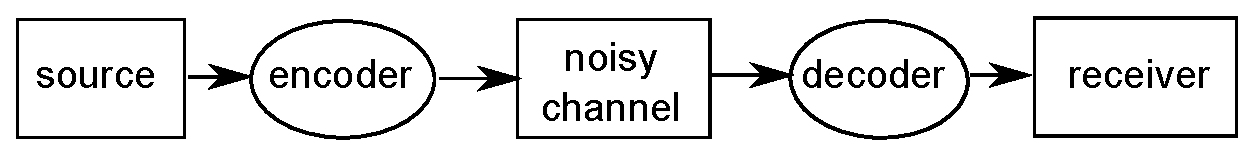
\includegraphics[width=0.8\linewidth]{pictures/comm-channel1.eps}
	\caption{The role of encoder and decoder.}
\end{figure}

The balance is found by the \emph{encoder}.
This entity takes the message from the source, modify it in some way, and transmit the result over the channel.
A \emph{decoder} is the entity that apply some transformation to the incoming flow of information before handling it to the receiver.
The decoder cannot perform the inverse of the encoder's function, because the channel applies noise to the information.
We will concentrate on the noisy channel, without considering encoder and decoder's interfaces to source and receiver.

%NOTE: here he said something on asimptotic equipartition

\section{\acl{DMC}}

For now, the channel is a black box.
Let $\X$ be the input alphabet and $\Y$ be the output alphabet for the strings that respectively enter and exit the channel.
Select an input symbol $x \in \X$; a random symbol $y \in \Y$ comes out of the channel.

We can think that there is a ``devil'' inside the black box.
The devil has dices that have $\abs{\Y}$ faces.
Whenever an input signal enters the channel, the devil launches a dice and outputs the symbol on the facet that comes up.
The devil cannot launch any dice he likes; instead, there is a mapping between dices and input symbols (you can think of $x$ as the name of the dice that the devil has to use).
So we can influence the devil in using some specific dice (out of the $\abs{\X}$ dices), but the outcome is still stochastic: the probability distribution of each dice is arbitrary.
Note that the channel is usable if we have different dices; otherwise, the output is completely uncontrollable.

Let $W(y|x)$ be the probability that the dice named $x$ will fall onto its facet $y$, with the following conditions: 
\begin{itemize}
	\item $W(y|x) \ge 0$,
	\item $\forall x . \sum_{y \in \Y} W(y|x) = 1$.
\end{itemize}
We can think of $W$ as a matrix whose columns are indexed by $y$ and rows are indexed by $x$.

To communicate iteratively pick $x_1, x_2, \dots, x_n \in \X^n$ and launch a sequence of dices.
There is a probability distribution for $y_1, y_2, \dots, y_n \in Y^n$. Consider the function
\begin{equation*}
	W^n : \X^n \to \Y^n,
\end{equation*}
defined as
\begin{equation*}
	W^n \left( \str{x}, \str{y} \right)
	= \prod_{i = 1}^n W \left( y_i | x_i \right).
\end{equation*}

We assume that every symbol is independently modified (lack of memory of the channel).
Our \ac{DMC} (over time instants) is defined by the set $\left\{ W^n \right\}_{n = 1}^{\infty}$.

\section{Shannon's Noisy Channel Theorem}

The encoder takes the messages of the source and maps it to an arbitrary subset $\C \subseteq \X^n$.
So we have $\abs{\C}$ many messages that can flow in the channel; they can be non-binary strings, but to have an approximation of their length we can assume they are binary.
Then, the length of these messages is $\logtwo{\abs{\C}}$.
We define the speed of the channel as
\begin{equation*}
	\frac{1}{n} \cdot \logtwo{\abs{\C}},
\end{equation*}
where $n$ is the length of transmission in some unit of time.
We can call this \emph{rate} of the code.

Now we are interested in the quality of transmission, that is how well data transmitted can be recovered.
The decoder is a function $\phi: \Y^n \to \C$.
An error event happens when $\str{x} \in \X^n$ is transmitted and $\phi(\str{y}) \neq \str{x}$ is received.
Define
\begin{equation*}
	W^n \left( T|\str{x} \right)
	=
	\sum_{\str{y} \in T} W^n \left( \str{y}|\str{x} \right),
\end{equation*}
where $T \subseteq \Y$.
The error probability of a string $\str{x} \in \X^n$ is
\begin{equation*}
	1 - W^n \left( \phi^{-1}(\str{x}) | \str{x} \right)
	=
	W^n \left( \overline{\phi^{-1}(\str{x})} | \str{x} \right),
\end{equation*}
where
\begin{equation*}
	\phi^{-1}(\str{x}) = \left\{ \str{y} : \phi(\str{y}) = \str{x} \right\}.
\end{equation*}

Define the (maximum) error probability of the code $(\C_n, \phi_n)$ ($W^n$ is fixed) as 
\begin{equation*}
	e_m \left( W^n, \C_n, \phi_n \right)
	=
	\max_{\str{x} \in \C} W^n \left( \overline{\phi^{-1}(\str{x})}, \str{x} \right).
\end{equation*}

\begin{prop}
	$R \geq 0$ is an \emph{achievable rate} of transmission over the \ac{DMC} $\{ W \}$ if exists $\{(\C_n, \phi_n)\}_{n=1}^\infty$ such that:
	\begin{itemize}
		\item $\lim_{n \to \infty} \frac{1}{n} \logtwo{\abs{\C_n}} \ge R$;
		\item $\lim_{n \to \infty} e_m(W, \C_n, \phi_n) = 0$.
	\end{itemize}
\end{prop}

What is the highest achievable rate?
\begin{equation*}
	\C \subseteq \X^n \implies \frac{1}{n} \logtwo{\abs{C}} \le \logtwo{\abs{\X^n}}.
\end{equation*}
So the maximum achievable rate is $\logtwo{\abs{\X^n}}$.
Also, if $R_t$ is a series of achievable rates and $R_t$ tends to $R$, then $R$ is an achievable rate too (simple analysis, will not be demonstrated).

Shannon wondered about the highest achievable rate $C(W)$ of a given DMC $\{W\}$.
He called this number \emph{capacity of the channel}.
The answer came out of his intuition but it has been proved true by his students and co-workers.

Let $x \in \X$ be a symbol chosen following a probability distribution $P|\X$.
The input symbol will be sent through the channel $W$ and the output is conditioned by $W$.
Let $Y$ be a \ac{RV} $Y \in \Y$ representing the output of $W$ with respect to input $X$.
Then, we have a joint distribution $P, W | \X \times \Y$.
The probability that a specific input $x$ corresponds to a received symbol $y$ is
\begin{equation*}
	\Pr{X = x, Y = y} = P(x) W(y|x).
\end{equation*}

Define $\MutualInformation{X \land Y}$ to be the number of bits that one can transmit over a channel in a unit of time.
Intuitively, it is what $y$ retains of input $x$ (mutual information).
We can maximize $I$ by controlling the probability distribution $P|\X$.
With some abuse of notation:
\begin{equation*}
	\max_{P|\X} \MutualInformation{P, W}.
\end{equation*}
What is the formula for $I$?
\begin{align*}
	\MutualInformation{X \land Y}
	& =
	\sum_{(x, y) \in \X \times \Y}
	\Pr{X=x, Y=y} \cdot
	\logtwo{\frac{\Pr{X=x, Y=y}}{\Pr{X=x} \cdot \Pr{Y=y}}}
	\\
	& =
	\sum_{x \in \X,  y \in \Y}
	\Pr{X=x} \cdot W(y|x) \cdot
	\logtwo{\frac{\Pr{X=x} \cdot W(y|x)}{\sum_{x \in X} \Pr{X=x} \cdot W(y|x)}}
	\\
	& =
	\MutualInformation{P, W}.
\end{align*}

\begin{thm}[Shannon's Noisy Channel Theorem]\label{thm:nct}
	The highest achievable rate, given a \ac{DMC} $W$, is
	\begin{equation*}
		C(w) = \max_{P|X} \MutualInformation{P, W}.
	\end{equation*}
\end{thm}

Notice that $C(W)$ is 0 if $X$ and $Y$ are independent, \ie all rows in $W$ are the same. 

\section{\acl{BSC}}

A \ac{BSC} is used to transmit binary strings and the \ac{DMC} has the form
\begin{equation*}
	W = 
	\begin{pmatrix}
		1-p & p \\
		p & 1-p
	\end{pmatrix},
\end{equation*}
with $\X = \Y = \{0,1\}$.

It is called symmetric because $W$ is symmetric.
In this context $P|\X$ is called \emph{crossover} probability.
The capacity of this channel according to \cref{thm:nct} is
\begin{equation*}
	\MutualInformation{X \wedge Y}
	=
	\Entropy{Y} - \Entropy{Y|X}
	\le
	1 - \entropy{p}.
\end{equation*}

This is true because:
\begin{itemize}
	\item the maximum value for $\Entropy{Y}$ is 1;
	\item the following equations hold:
		\begin{equation*}
			\Entropy{Y | X} =
			\sum_{x \in \X} \Pr{X = x} \cdot \Entropy{Y | X = x} =
			\entropy{p},
		\end{equation*}
		where
		\begin{equation*}
			\Entropy{Y | X = x} =
			\sum_{y \in \Y} \Pr{Y = y | X = x} \cdot
			\logtwo{\frac{1}{\Pr{Y = y | X = x}}}.
		\end{equation*}
\end{itemize} 

Is this upper bound achievable? We must make sure that
\begin{equation*}
	\exists X : \Entropy{Y} = 1.
\end{equation*}
We can impose the uniform distribution when picking the input values, \ie $\Pr{X = 0} = \frac{1}{2}$.

\begin{obs}
	$1-\entropy{2p}$ is an achievable rate if $p < \frac{1}{4}$.
\end{obs}
We will do this using error correcting codes.

\begin{proof}
	Choose arbitrary $\str{x} \in \{0, 1\}^n$, but think of $\zero$ (it's easier).
	Consider the Hamming ball $\hball{\zero}{n(p+\epsilon)}$; we want that
	\begin{equation*}
		W^n \left( \phi^{-1}_n(\zero) | \zero \right) \to 1.
	\end{equation*}
	Consider a code for which
	\begin{equation*}
		\forall \str{x} \in \C_n .
		\phi^{-1}_n(\str{x}) \supseteq \hball{\str{x}}{n(p+\epsilon)};
	\end{equation*}
	these Hamming balls should be disjoint.
	We wonder if it is true that
	\begin{equation*}
		W^n \left( \hball{\zero}{n(p+\epsilon)} | \zero \right) \to 1.
	\end{equation*}
	This is what we should achieve, and prove that $np$ is a good choice.
	What we receive is $\str{x} \xor Z^n$, for some \ac{RV} $Z^n$, defined as $Z^n = \str{x} \xor Y^n$.
	\begin{equation*}
		Y^n \in \hball{\zero}{n(p+\epsilon)} \iff Z^n \text{ has at most } n(p+\epsilon) \text{ 1s}. 
	\end{equation*}

	The number of 1s in $Z^n$ is equal to $\sum_{i = 1}^{n} Z_i$, where $Z_i \sim (1-p, p)$ is a \ac{RV}.

	\begin{equation*}
		\expectation{Z_i} = \Pr{Z_i = 0} \cdot 0 + \Pr{Z_i = 1} \cdot 1 = p.
	\end{equation*}

	$\{Z_i\}_{i=1}^n$ is an \ac{IID} sequence of \acp{RV}.
	\begin{equation*}
		\expectation{Z^n} =
		\expectation{\sum_{i = 1}^{n} Z_i} =
		\sum_{i = 1}^{n} \expectation{Z_i} =
		n \cdot p.
	\end{equation*}

	By the law of large numbers,
	\begin{equation*}
		\Pr{\abs{\frac{1}{n} \sum_{i = 1}^{n} Z_i - p} > \epsilon} \to 0.
	\end{equation*}
	The complement of this event has a probability that converges to 1.
	How can we guarantee that these Hamming balls of radius $n(p+\epsilon)$ are disjoint?
	This is guaranteed if $\hdist{\str{x}',\str{x}''} \ge 2n (p+\epsilon)$.
	Thus $\hdist{\C_n} \ge 2n(p+\epsilon)$.
	The Gilbert-Varhsamov bound (\cref{thm:gilbert-varshamov}) says that, if $\delta < \frac{1}{2}$,
	\begin{equation*}
		\exists \C_n : \abs{\C_n} \gtrsim 2^{n \, (1-\entropy{\delta})},
	\end{equation*}
	and that
	\begin{equation*}
		\hdist{\C_n} \gtrsim n \delta.
	\end{equation*}

	We want that $d_H(\C_n) \ge 2n(p+\epsilon)$, thus what we want is achievable if and only if
	\begin{equation*}
		2p + \epsilon < \dfrac{1}{2} \sim p < \dfrac{1}{4}. \qedhere
	\end{equation*}
\end{proof}

Shannon stated something stronger, namely that the capacity is $1 - \entropy{p}$.
Shannon uses ``maximum likelihood''.
He chooses $2^{n \, R}$ strings at random from $T^n_p$, given $P|\X$.

\begin{thm}[Converse part of Shannon's noisy channel coding theorem]
	If $R$ is such that $\exists \{\C_n, \phi_n\}_{n=1}^\infty$ with
	\begin{equation*}
		\limsup_{n \to \infty}
		\frac{1}{n} \cdot \logtwo{\abs{\C_n}} \ge R,
	\end{equation*}
	and
	\begin{equation*}
		\lim_{n \to \infty} e_n (W^n, \C_n, \phi) = 0,
	\end{equation*}
	then
	\begin{equation*}
		R \le \max_{
			\substack{
				X \in \X : \\
				P_{Y|X} = W
			}
		}
		\MutualInformation{X \land Y}.
	\end{equation*}
\end{thm}

\begin{proof}
	Let $M_n$ be a \ac{RV} uniformly distributed over $\C_n$.
	Take $\frac{1}{n} \cdot \Entropy{M_n}$, the average entropy.
	\begin{equation*}
		\frac{1}{n} \cdot \Entropy{M_n} =
		\frac{1}{n} \cdot \logtwo{\abs{\C_n}}.
	\end{equation*}
	To get the upper bound, we manipulate the \ac{LHS}.
	\begin{equation*}
		\frac{1}{n} \cdot \Entropy{M_n} =
		\frac{1}{n} \cdot \left[ \Entropy{M_n} - \Entropy{M_n | \phi_n(Y^n)} \right] +
		\frac{1}{n} \cdot \Entropy{M_n | \phi_n(Y^n)},
	\end{equation*}
	where $Y^n$ is the \ac{RV} defined by $P_{Y^n | M_n} = W^n$.
	In the square brackets we have a mutual information, so
	\begin{equation*}
		\frac{1}{n} \cdot \Entropy{M_n} =
		\frac{1}{n} \cdot \MutualInformation{M_n \land \phi_n(Y^n)} +
		\frac{1}{n} \cdot \Entropy{M_n | \phi_n(Y^n)}.
	\end{equation*}
	We should be able to prove that this is not more than the upper bound.
	We expect the other therm to be negligible; with high probability the result of decoding the received codeword is the codeword that was sent.
	\begin{equation*}
		\MutualInformation{M_n \land \phi_n(Y^n)} \le
		\MutualInformation{M_n \land Y^n}.
	\end{equation*}
	This is from the fact that information cannot be gained by processing the \acp{RV}.
	We see this by looking at
	\begin{equation} \label{eq:dis1}
		\MutualInformation{M_n \land \phi_n(Y^n)} \le
		\MutualInformation{M_n \wedge \phi_n(Y^n), Y^n},
	\end{equation}
	since
	\begin{equation*}
		\Entropy{M_n} - \Entropy{M_n | \phi_n(Y^n)} \le
		\Entropy{M_n} - \Entropy{M_n | \phi_n(Y^n), Y^n},
	\end{equation*}
	and since
	\begin{equation*}
		\Entropy{M_n | \phi_n(Y^n)} \ge
		\Entropy{M_n | \phi_n(Y^n), Y^n},
	\end{equation*}
	\Cref{eq:dis1} follows.

	The \ac{RHS} of \cref{eq:dis1} can be written as
	\begin{align*}
		\MutualInformation{M_n \land \phi_n(Y^n), Y^n}
		& =
		\MutualInformation{M_n \land Y^n} +
		\MutualInformation{M_n \land \phi_n(Y^n) | Y^n}
		\\
		& =
		\MutualInformation{M_n \land Y^n}.
	\end{align*}
	we see that
	\begin{equation*}
		\MutualInformation{M_n \land \phi_n(Y^n) | Y^n} \le
		\Entropy{\phi_n(Y^n) | Y^n} = 0.
	\end{equation*}

	So we obtain the following inequality:
	\begin{equation*}
		\MutualInformation{M_n \land \phi_n(Y^n)} \le
		\MutualInformation{M_n \land Y^n}.
	\end{equation*}
	As notation, $M_n = X_1 \dots X_n$ is a vector of \acp{RV}.
	Thus,
	\begin{equation*}
		\MutualInformation{M_n \land Y^n} =
		\MutualInformation{X^n \land Y^n}.
	\end{equation*}
	This is what we want to upper bound with the conjectured value of capacity.
	We write
	\begin{equation*}
		\MutualInformation{X^n \land Y^n} =
		\Entropy{Y^n} - \Entropy{X^n | Y^n} \le
		\sum_{i = 1}^n \Entropy{Y_i} - \Entropy{Y^n | X^n}.
	\end{equation*}
	For $\Entropy{Y^n | X^n}$ we use the chain rule:
	\begin{equation*}
		\Entropy{Y^n | X^n} =
		\sum_{i = 1}^n \Entropy{Y_i | X^n, Y_1, \dots, Y_{i-1}}.
	\end{equation*}

	But in a \ac{DMC} we have that
	\begin{equation*}
		\Entropy{Y_i | X^n, Y_1, \dots, Y_{i-1}} =
		\Entropy{Y_i | X_i},
	\end{equation*}
	so
	\begin{equation*}
		\Entropy{Y^n | X^n} = \sum_{i = 1}^{n} \Entropy{Y_i | X_i}.
	\end{equation*}

	So what we get is that
	\begin{equation*}
		\MutualInformation{X^n \land Y^n} =
		\sum_{i = 1}^{n} \MutualInformation{X_i \land Y_i}.
	\end{equation*}
	This is true because our channel is a particular type of channel.

	\begin{equation*}
		\sum_{i = 1}^{n} \MutualInformation{X_i \land Y_i} \le
		n \cdot \max_{P_{Y|X} = W} \MutualInformation{X \land Y}.
	\end{equation*}
	which is $n$ times capacity.
	So:
	\begin{equation*}
		\frac{1}{n} \cdot \MutualInformation{M_n \land \phi_n(Y^n)} \le C(W).
	\end{equation*}

	For the second part, we have to prove that 
	\begin{equation*}
		\frac{1}{n} \cdot \Entropy{M_n | \phi_n(Y^n)} \to 0.
	\end{equation*}

	We do so using Fano's inequality.
	We introduce the \ac{RV} $Z_n$ defined as
	\begin{equation*}
		Z_n =
			\begin{cases}
				1 \text{ if } \phi_n(Y^n) \neq M_n,\\
				0 \text{ otherwise.}
			\end{cases} 
	\end{equation*}

	We can say that
	\begin{equation*}
		\Entropy{M_n | \phi_n(Y^n)} \le
		\Entropy{M_n, Z_n | \phi_n(Y^n)}
	\end{equation*}
	since we ``added'' something to a \ac{RV}.

	\begin{align*}
		\Entropy{M_n, Z_n | \phi_n(Y^n)}
		& =
		\Entropy{Z_n | \phi_n(Y^n)} +
		\Entropy{M_n | \phi_n(Y^n), Z_n}
		\\
		& \le
		\Entropy{Z_n} +
		\Entropy{M_n | \phi_n(Y^n), Z_n}
		\\
		& \le
		1 +
		\Entropy{M_n | \phi_n(Y^n), Z_n}.
	\end{align*}
	So for now we have that
	\begin{equation*}
		\frac{1}{n} \cdot \Entropy{M_n | \phi_n(Y^n)} \le
		\frac{1}{n} + \frac{1}{n} \cdot \Entropy{M_n | \phi_n(Y_n), Z_n}.
	\end{equation*}
	We have to show that
	\begin{equation*}
		\frac{1}{n} \cdot \Entropy{M_n | \phi_n(Y_n), Z_n}
	\end{equation*}
	is small.
	We can break this up:
	\begin{equation} \label{eq:eqbreak}
	\begin{aligned}
		\frac{1}{n} \cdot \Entropy{M_n | \phi_n(Y_n), Z_n}
		= &~
		\Pr{Z_n = 1} \cdot \Entropy{M_n | \phi_n(Y^n), Z_n = 1} +
		\\
		&~+
		\Pr{Z_n = 0} \cdot \Entropy{M_n | \phi_n(Y^n), Z_n = 0}.  
	\end{aligned}
	\end{equation}
	Now we have to bring in the error probability.
	\begin{align*}
	  \epsilon_n
	  & =
	  \Pr{Z_n = 1} =
	  \Pr{M_n \neq \phi_n(Y^n)}
	  \\
	  & \le
	  e_n(W^n, \C_n, \phi_n) \to 0.
	\end{align*}
	So $\epsilon_n \to 0$, since the average is not more than the maximum.
	\begin{align*}
		\Entropy{M_n | \phi_n(Y^n), Z_n = 1}
		& =
		\\
		\sum_{y \in \Y^n} \Pr{Y^n = y}
		& \cdot
		\Entropy{M_n | \phi_n(Y^n) = \phi_n(y), Z_n = 1}.
	\end{align*}

	$M_n \in \X^n$.
	So that entropy is less than $\logtwo{\abs{\X^n}}$.
	So the first term of \cref{eq:eqbreak} can be bounded by
	\begin{equation*}
		\epsilon_n \cdot
		\frac{1}{n} \cdot
		\Entropy{M_n | \phi_n(Y^n), Z_n = 1} \le
		\epsilon_n \cdot
		\frac{1}{n} \cdot
		\logtwo{\abs{\X^n}} =
		\epsilon_n \cdot \logtwo{\abs{\X}} \to 0.
	\end{equation*}
	The second term of \cref{eq:eqbreak} is equal to 0.
	\begin{equation*}
		\frac{1}{n} \cdot \Pr{Z_n = 0} \cdot \Entropy{M_n | \phi_n(Y^n), Z_n = 0}.
	\end{equation*}
	To see why, note that there is no error, so $M_n = \phi_n(Y^n)$.
\end{proof}


\section{Zero Error Capacity}
Zero stands for zero probability, so the probability of error is bound to be equal to 0. We translate this problem in graph theory: we will look
at product of graphs and powers of graphs. We have a DMC $\{W\},\ W:\X \rightarrow \Y$. $W^n:\X^n \rightarrow \Y^n$, the mathematical model of a code is the very same. A code is $(\C_n, \phi)$ with $\C_n \subseteq \X^n$ and $\phi: \Y^n \rightarrow \C_n$. A code has two parameters:

\begin{itemize}
	\item $\dfrac{1}{n}|\C_n|$ is the size of the code compared to $n$. It is the number of bits transmitted over the channel per use of the channel.
	\item $e_n(W^n, \C_n, \phi) = \max_{\str{x} \in \C_n} W^n(\overline{\phi^{-1}(\str{x})}|\str{x})$ is the probability of error.
\end{itemize}

$(\C_n, \phi)$ is a zero error code if $e_n(W^n, \C_n, \phi)=0$. $R \geq 0$ is an achievable rate for error probability $0$ if $\exists (\C_n, \phi_n)$, $\C_n \subseteq \X^n$ with
\[
\overline{\lim_{n \rightarrow \infty}} \dfrac{1}{n}\log|\C_n| \geq R\text{ and }
\]

\[
e_n(W^n, \C_n, \phi_n) = 0.
\]

If $W(y|x) > 0$ for all $x, y$ then this is not possible. If you have 0s in the matrix, we are only interested in the patterns of the 0s. To have 0 error, we should have that
\[
W^n(\phi^{-1}(\str{x})|\str{x}) = 1,\ \forall\str{x} \in \C_n
\]

The decoding function must be fixed if we want $0$ error. If $W^n(\str{y}|\str{x}) \geq 0$, we must have that $\phi^{-1}(\str{y}) = \str{x}$. Given $\str{x}$, the set $\{\str{y}| W^(\str{y}|\str{x})>0 \}$ is uniquely defined. This is the support of conditional distribution:
\begin{equation}
\supp(\str{x}) = \{\str{y}| W^n(\str{y}|\str{x})>0 \}
\end{equation}

We should have that 
\[
\supp(\str{x}) \subseteq \phi^{-1}(\str{x}),\ \forall\str{x} \in \C_n
\]

So this,\ie how to get the 0 error probability, only depends on the set $\C_n$. Support sets have to be disjoint. $\C_n$ is a $0$ error code if
\[
\forall \{\str{x}',\str{x}'' \} \in \binom{\C_n}{2}\ \supp(\str{x}') \cap \supp(\str{x}'') = \emptyset
\]

\begin{obs}
	Let $\str{x} \in \X^n$. Then $$\str{y} \in \supp(\str{x}) \Leftrightarrow W^n(\str{y}|\str{x}) >0,$$ but $W^n$ is a product of probabilities; thus, since
	$$W^n(\str{y}|\str{x}) = \prod_{i=1}^nW(y_i|x_i)$$
	it must be that
	$$W(y_i, x_i) > 0,\ \forall i.$$ So the support set is $$\supp(\str{x}) = \times_{i=1}^n\supp(x_i)$$
\end{obs}

This is a combinatorial condition. The support is the set of positive elements of the row of $x$. You need at least two orthogonal rows in the matrix.

\begin{obs}
	$$\supp(\str{x}') \cap \supp(\str{x}'') = \emptyset \Leftrightarrow \supp(x_i') \cap \supp(x_i'') = \emptyset,$$ for some $i$. 
\end{obs}
\noindent\textbf{Proof}. Suppose 
\begin{align*}
	&\supp(\str{x}') \cap \supp(\str{x}'') \not= \emptyset\\
	&\Leftrightarrow \exists\str{z} \in \supp(\str{x}') \cap \supp(\str{x}'')\\
	& \Leftrightarrow z_i \in \supp(x') \cap \supp(x''),\ \forall i
\end{align*}
$\hfill\Box$

Consider the graph $G = G(W)$ such that $V(G) = \X$ and $\{x',x'' \} \in E(G)$ if $\supp(x') \cap \supp(x'') = \emptyset$. We are looking for a clique in this graph, which is the size of the best code one can have $\omega(G)$ (?) What about when we use the channel more than once? We look at $G^n = G(W^n)$, where $V(G^n) = \X^n$ and $\{\str{x}',\str{x}''\} \in E(G^n)$ if $\exists i\ \supp(x_i') \cap \supp(x_i'') = \emptyset$. This sequence of graphs can be built using the first graph, not using always the matrix.

\noindent From $G$ to $G^n$.

\noindent Take $G$. If $\{a, b\} \in E(G)$ they are indistinguishable. Now take $G^n$. $\{\str{a}, \str{b}\} \in E(G^n)$ are indistinguishable if $\exists i \{a_i, b_i\} \in E(G)$ with $a = a_1\ldots a_n$ and $b=b_1\ldots b_n$. Every clique of maximal length is a 0 error code.

We say that 
\[
\overline{\lim_{n \rightarrow \infty}}\dfrac{1}{n}\log \omega(G^n)
\]

is the zero error capacity of $G$. This limit exists for every graph.

\begin{prop}
	For every graph $G\ \exists W\ s.t.\ G = G(W)$.
\end{prop}

Consider a matrix $W$ where the rows are the vertexes of the graphs and columns are indexed by the non-edges, \ie the pairs of $\binom{V(G)}{2}$ that are not in $E(G)$.

\begin{equation}
	W(\{a,b\}|x) = \begin{cases}
	0\ if\ x\not\in \{a, b\}\\
	1\ if\ x\in \{a, b\}
	\end{cases}
\end{equation}

If the rows of $x$ and $y$ are not orthogonal, $\{x, y\}$ is not an edge. There are two problems:
\begin{itemize}
	\item rows could not sum to 1;
	\item rows could sum up t 0.
\end{itemize}

The first problem is avoided by dividing the rows. The second is a avoided by doing
\[
W = (W\ I)
\]

then $W$ can be normalized. Now $G = G(W)$.

$\hfill\Box$

$ \sqrt[n]{\omega(G^n)}$ is how much larger is $\omega(G^n)$ with respect to $\omega(G)$. For graphs of $5$ vertices there is only one graph for which
\[
 \sqrt[n]{\omega(G^n)} \not=\omega(G),
\]
it is the following.
\begin{figure}[h!]
	\centering
	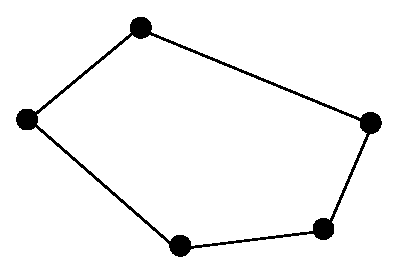
\includegraphics[width=100px]{pictures/graph5v.eps}
\end{figure}

Lovàsz gave a function for $ \sqrt[n]{\omega(G^n)}$ in '79. In fact it works for graphs that are self complementary and vertex transitive.

\begin{equation}
	C(G) = \overline{\lim_{n\rightarrow \infty}}  \sqrt[n]{\omega(G^n)}
\end{equation}

Shannon proved that
\[
\sqrt{5} \leq C(C_5) \leq \dfrac{5}{2}
\]

Lovàsz proved that in fact $C(C_5) = \sqrt{5}$. For the upper bound we have that $C_5 = G(W)$ with
\[
 W = \left(\begin{array}{c c c c c}
 \frac{1}{2} &\frac{1}{2} & 0&0&0\\
 0&0&\frac{1}{2}&\frac{1}{2}&0\\
 \frac{1}{2}&0&0&0&\frac{1}{2}\\
 0&\frac{1}{2}&\frac{1}{2}&0&0\\
 0&0&0&\frac{1}{2}&\frac{1}{2}\\
 \end{array}\right)
\]

then said that 0 error capacity is less than or equal to the capacity. Shannon noticed, for the lower bound, that $C(G) > \omega(G)$, but $\omega(G) = 2$. If you look at $G^2$, \ie $C_5^2$, then $\omega(C_5^2) = 5$.
\[
\omega(G^n) \geq [\omega(G)]^n
\]
with the product set you get $4$. But Shannon noticed that those $5$ strings are distinguishable:
\[
\{00,11,24,31,43\}.
\]
\[
 \sqrt[n]{\omega(G^n)} \geq \omega(G)
\]
\[
 C(G) = \overline{\lim_{n\rightarrow \infty}}\sqrt[n]{\omega(G^n)}
\]
That is, Shannon capacity of G.

\begin{lem}[Fevete]
Take a sequence of reals $a_n \in \Reals$, if the sequence id super additive, $\ie\ a_{m+n} \geq a_m + a_n\ \forall m, n \in \mathbb{N}$ and
\[
 \dfrac{a_n}{n} \leq M\ \forall n \in \mathbb{N}
\]

then
\[
 \exists \lim_{n \rightarrow \infty}  \dfrac{a_n}{n} 
\]

and

\[
\lim_{n \rightarrow \infty}  \dfrac{a_n}{n} = \sup_n \dfrac{a_n}{n}. 
\]
 
\end{lem}

To apply this to $\omega(G^n)$ we have to take the logarithm, since $\omega(G^n)$ is super multiplicative (and thus $\log(\omega(G^n))$ is super additive). We have that $\omega(G^n) \leq |V(G)|^n$, and thus
\[
 \dfrac{\log(\omega(G^n))}{n} \leq \log|V(G)|
\]

since 

\[
 \dfrac{a_n}{n} \leq M,\ \exists \hat{M} = \sup_n \dfrac{a_n}{n}\ \text{with}\ \hat{M} \leq M,
\]

so
\[
 \forall \epsilon\ \exists n_0\ \dfrac{a_{n_0}}{n_0} > \hat{M} - \epsilon.  
\]

Take arbitrary $n > n_0$ with $n = q_nn_0 +r_n$, with $0 \leq _n < n_0$.

\begin{align*}
 \dfrac{a_n}{n} = \dfrac{a_{q_nn_0 +r_n}}{q_nn_0 +r_n} & \geq \dfrac{q_na_{n_0} +a_{r_n}}{(q_n+1)n_0}\\
 & = \dfrac{q_n}{q_{n+1}} \dfrac{a_{n_0}}{n_0} + \dfrac{a_{r_n}}{(q_n + 1)n_0}.
\end{align*}

so the limit can be bounded from below

\[
 \underline{\lim_{n\rightarrow \infty}} \dfrac{a_n}{n} \geq \underline{\lim_{n\rightarrow \infty}}\left(\dfrac{q_n}{q_{n+1}} \dfrac{a_{n_0}}{n_0} + \dfrac{a_{r_n}}{(q_n + 1)n_0}\right) \geq \hat{M} - \epsilon
\]

(since $a_{r_n} \geq \min\{a_0, \ldots,a_{n_0 -1}\}$ the last fraction goes to 0).

$\hfill\Box$

\begin{prop}
 $$\omega(G) \leq C(G) \leq \chrom{G},$$ where $\chrom{G}$ is the chromatic number of $G$.
\end{prop}

A colouring of $G$ is a function $f: V(G) \rightarrow C$ such that if $\{a, b\} \in E(G)$ then $f(a) \not= f(b)$. $\chrom{G}$ is the minimum cardinality of $C$ such that a function $f: V(G) \rightarrow C$ like that exists.

\noindent\textbf{Proof}. 
\[
 [\omega(G)]^n \leq \omega(G^n) \leq \chrom{G^n}
\]

the first part comes from super-multiplicativity of $\omega(G)$, the second from the fact that the chromatic number of a graph is greater than the largest clique. Since $\chrom{G}$ is sub-multiplicative, we have $$\chrom{G^n} \leq [\chrom{G}]^n.$$

To show that $\chrom{G}$ is sub-multiplicative, consider an optimal colouring of $G$. $$f:V(G) \rightarrow C\ \text{with}\ |C| = \chrom{G}$$ take $\str{x} \in V(G^n)$, we colour it separately, for $x_i$ in $x_1\ldots x_n$. The function $f^n(\str{x})$, the extension by concatenation, id a correct colouring. If $\{\str{x}, \str{y}\} \in E(G^n)$, it must be that $\exists i : \{x_i, y_i\} \in E(G)$, but then, since $f(x_i) \not=f(y_i)$, $f^n(\str{x}) \not= f^n(\str(y))$. Also, the number of colours used by $f^n$ id no more than $|C^n| = [\chrom{G}]^n$, so
\[
 \omega(G) \leq \sqrt[n]{\omega(G^n)} \leq \chrom{G}
\]

$\hfill\Box$

[Note: There is a simple upper bound that is better than this. You use the ``fractional'' chromatic number. You express colouring as PU (?) and drop integer constant.]

\begin{cor}
 $$\omega(G) = \chrom{G} \Rightarrow C(G) = \omega(G).$$
\end{cor}

The corollary doesn't give us much. You can make any graph like this. Schutzenberger + Berge showed some classes of graphs for which this holds. One example is graphs for which vertices are intervals, and intersecting intervals share and edge. Furthermore, $\forall G' \subseteq G$ induced $\omega(G') = \chrom(G')$, for interval graphs.

\begin{definition}[Perfect graph]
 $G$ i perfect if $$\omega(G') = \chrom{G'}\ \forall G' \subseteq G,$$ where $G'$ is an induced subgraph.
\end{definition}

What makes this definition beautiful are two conjectures, by Berge. By now they are both theorems.
\begin{itemize}
 \item \textbf{Weak}: $G$ is perfect $\Leftrightarrow \overline{G}$ is perfect.
 \item \textbf{Strong}: minimally imperfect graphs are either odd cycles or their complements.
\end{itemize}

\begin{definition}[Minimally imperfect graph]
 A graph $G$ is minimally imperfect if
 \begin{enumerate}
  \item $G$ is not perfect, \ie $\omega(G) < \chrom{G}$,
  \item $\forall G' \subseteq G$ induced subgraph, $G'$ is perfect, \ie $\omega(G') = \chrom{G'}$.
 \end{enumerate}

\end{definition}





\end{document}
